\documentclass[11pt]{report}

% ---------- Layout ----------
\usepackage[margin=1in]{geometry}
\usepackage[utf8]{inputenc}
\usepackage[english]{babel}
\usepackage{amsmath,amssymb}
\usepackage{longtable}

% ---------- Graphics & Colors ----------
\usepackage{graphicx}
\usepackage{xcolor}

% Branding colors (pick one set of values and keep it consistent)
\definecolor{qcRed}{HTML}{E22237}   % Snapdragon Red
\definecolor{qcDark}{HTML}{101820}  % Dark neutral
\definecolor{qcGray}{HTML}{EDEDED}  % Light gray (optional)

% ---------- Utility Macros (branding) ----------
\newcommand{\qcrule}{\textcolor{qcRed}{\rule{16cm}{5pt}}}
\newcommand{\qctitle}[1]{\textcolor{qcRed}{\Huge\bfseries #1}}
\newcommand{\qcsectiontitle}[1]{\textcolor{qcDark}{\Large\bfseries #1}}

% ---------- Fonts & Headings ----------
\usepackage{titlesec}

% Chapter: inline style "1. Document Information"
\titleformat{\chapter}[hang]
  {\normalfont\huge\bfseries\color{qcRed}}
  {\thechapter.}
  {1em}
  {}
\titlespacing*{\chapter}{0pt}{-5pt}{15pt}

% Section formatting
\titleformat{\section}
  {\normalfont\Large\bfseries\color{qcDark}}
  {\thesection}
  {1em}
  {}
\titleformat{\subsection}
  {\normalfont\large\bfseries\color{black}}
  {\thesubsection}
  {1em}
  {}
\titleformat{\subsubsection}
  {\normalfont\normalsize\bfseries\color{black}}
  {\thesubsubsection}
  {1em}
  {}

% ---------- Tables / Lists ----------
\usepackage{array}
\usepackage{longtable}
\usepackage{booktabs}
\usepackage{enumitem}
\usepackage{enumitem}
\setlist[itemize]{topsep=2pt, partopsep=0pt, itemsep=2pt, parsep=0pt}
\setlist[enumerate]{topsep=2pt, partopsep=0pt, itemsep=2pt, parsep=0pt}

% ---------- TOC styling ----------
\usepackage{tocloft}
\renewcommand{\cfttoctitlefont}{\huge\bfseries\color{qcRed}} % TOC title red
\renewcommand{\cftchapfont}{\color{qcRed}}      % chapter entries red
\renewcommand{\cftchappagefont}{\color{qcRed}}  % chapter page numbers red
\renewcommand{\cftsecfont}{\color{black}}       % sections black
\renewcommand{\cftsecpagefont}{\color{black}}
\renewcommand{\cftsubsecfont}{\color{black}}    % subsections black
\renewcommand{\cftsubsecpagefont}{\color{black}}

% ---------- Hyperlinks (load LAST among most packages) ----------
\usepackage[hidelinks]{hyperref}
\usepackage{bookmark}
\hypersetup{
    pdfsubject={Driver Safety AI on Snapdragon},
    pdfkeywords={Snapdragon, Qualcomm, On-device AI, Driver Monitoring, Drowsiness Detection},
    colorlinks=false,
    linktoc=all,
    pdfstartview=FitH,
    bookmarksopen=true,
    bookmarksnumbered=true
}

%Cover Page
% (pdfpages already loaded above indirectly; ensure single load and avoid
% duplicate hyperref loading to keep PDF bookmarks stable)
\usepackage{pdfpages}
\newcommand{\req}[1]{\hyperlink{#1}{\texttt{#1}}} % inline link macro


% ---------- Your Vars ----------
\def\myversion{1.0}

\setcounter{secnumdepth}{3}  % Number down to \subsubsection
\setcounter{tocdepth}{3}     % Include in the Table of Contents (optional)
\usepackage{float}

\usepackage[utf8]{inputenc}
\DeclareUnicodeCharacter{2265}{$\ge$}


\begin{document}

% --- Capstone cover page (from PDF) ---
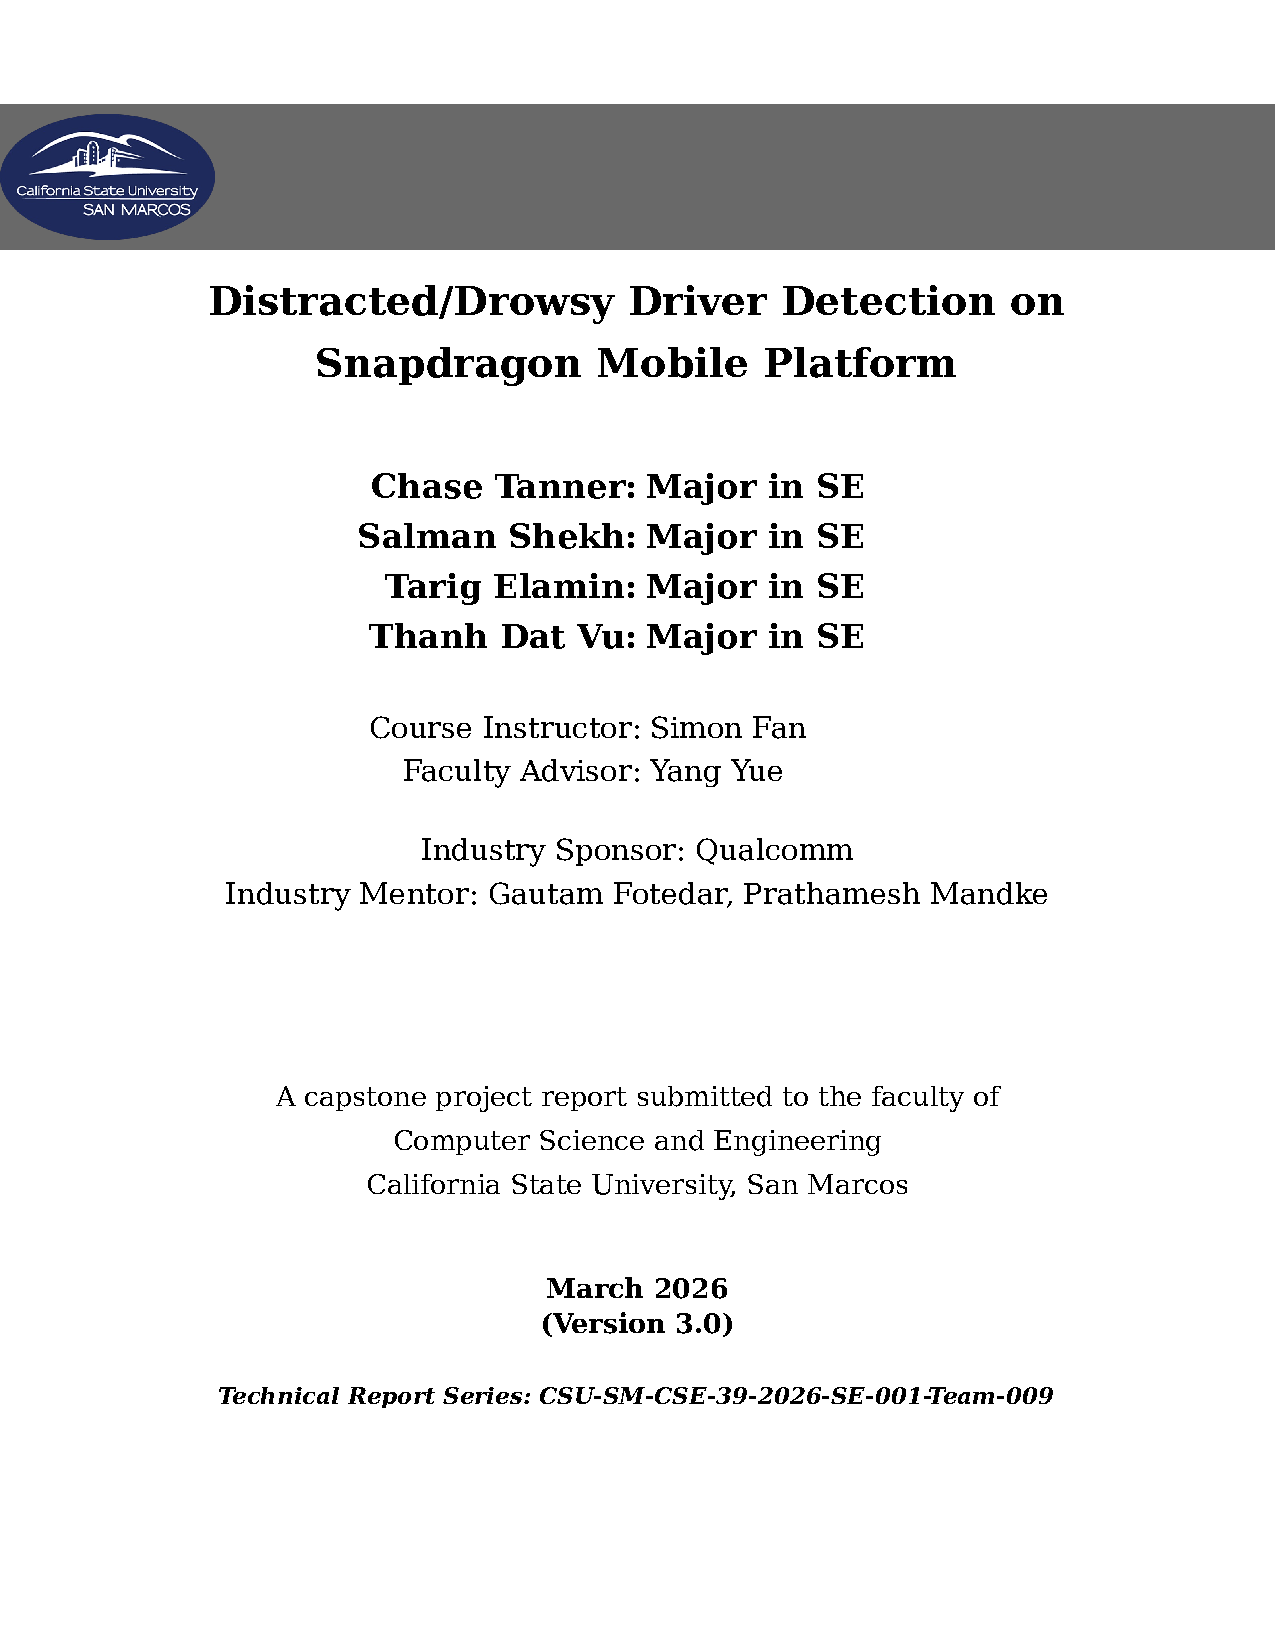
\includepdf[
  pages=1,                       % just the first page of the PDF
  pagecommand={\thispagestyle{empty}}, % ensure no headers/footers/bookmarks on cover
  fitpaper=true,                 % scale to full page
]{assets/CSU-SM-CSE-39-2026-SE-001-Team-009.pdf}

\clearpage

% reset numbering to start after the cover
\pagenumbering{arabic}
\setcounter{page}{1}



% ========================= TOC =========================
\tableofcontents
{\color{qcRed}\rule{16cm}{2pt}}

\clearpage

% ========================= Abstract =========================
\chapter{Abstract}
\textit{ALVION} is an Android application that detects signs of driver drowsiness and distraction using the phone’s front-facing camera and on-device computer vision. Many new vehicles include driver-monitoring features, but millions of older cars do not. Our goal is to help close that gap with a low-cost, widely accessible solution that can run on everyday Android devices and provide timely safety alerts during real driving.
In addition to being a prototype safety application, ALVION serves as a practical testbed to evaluate the real-world capability of Qualcomm-enabled mobile AI for this use case. We focus on whether mobile vision models and on-device acceleration are strong and stable enough to support driver-monitoring signals under realistic conditions (lighting changes, head movement, brief tracking loss, and different mounting angles). These findings help inform what is feasible today on commodity smartphones and what improvements are needed for more robust edge-based driver safety systems.
The system analyzes live video to extract visual cues related to fatigue and inattention, applies configurable thresholds and time-based logic, and triggers clear alerts through sound, on-screen prompts, and vibration when attention appears to drift. While core detection runs on-device for low latency, the application also includes standard product features such as user authentication (e.g., Firebase) to support a realistic app workflow. We do not attempt vehicle integration, cloud-based video processing, large-scale deployment, or regulatory certification.
This document outlines the project’s objectives, assumptions, and boundaries so developers, mentors, and faculty can stay aligned as the system evolves from concept to implementation. It describes the architecture, component responsibilities, and design decisions with an emphasis on building something practical within an academic timeline and extensible for future teams.

% ========================= DOC INFO =========================
\chapter{Document Information}

\section{Report Revision History}

\renewcommand{\arraystretch}{1.15}
\setlength{\tabcolsep}{6pt}

\begin{longtable}{|p{2cm}|p{3cm}|p{7.8cm}|p{3cm}|}
    \hline
    \textbf{Version} & \textbf{Date} & \textbf{Description} & \textbf{Author} \\
    \hline
    \endfirsthead

    \hline
    \textbf{Version} & \textbf{Date} & \textbf{Description} & \textbf{Author} \\
    \hline
    \endhead

    \hline
    \endfoot

    \hline
    \endlastfoot

    1.0 & Oct 13, 2025 &
    Initial draft submitted. Report outline aligned to capstone guidelines; 200--300 word abstract finalized; Introduction completed (Purpose, Background, Scope, Intended Audience, Project Description). Scope and constraints defined for on-device Snapdragon prototype. Document meta-setup added (revision history and approval tables). &
    Team 9 \\
    \hline

    1.5 & Oct 31, 2025 &
    Revised structural and behavioral design placeholders per faculty feedback; added preliminary UML comments, ERD rationale, and UI mockups for Version~2.0 preparation. Corrected terminology in diagrams, added reviewer annotations, and aligned architecture descriptions with grading criteria. Updated formatting, captions, and figure explanations for clarity and consistency. &
    Team 9 \\
    \hline

    2.0 & Dec 1, 2025 &
    Completed full capstone design document. Expanded all Requirements; finalized Architecture, Structural, and Behavioral Designs (MVC diagram, class diagrams, ERD, sequence and state diagrams); added UI mockups; completed Exploratory Studies, System Implementation, and System Testing sections including test framework setup and test-case definitions. Prepared new appendices (Appendix~T, Appendix~TE) for formal test cases. &
    Team 9 \\
    \hline

    2.5 & Dec 8, 2025 &
    Addressed instructor comments on context/scope diagrams, user--use-case cross-references, non-functional requirement grouping, and algorithm complexity; polished figures and layout. &
    Team 9 \\
    \hline

    3.0 & Feb 28, 2026 &
    Revised report to reflect updated user requirements and system development changes; confirmed system designs documented in Section~6 and added/updated most test case designs and execution reports in Section~8; revised Sections~1--5, 7, 9, and all appendices to align with the latest agile iteration; incorporated changed/new user requirements into refined system requirements and updated system design. &
    Team 9 \\
\end{longtable}

\clearpage

% ========================= 3. PROBLEM & CONTEXT =========================
\chapter{Problem Statement}


\section{Business Background}
Driver monitoring is becoming a regulatory and industry standard for road safety. The European Union now mandates such systems in new vehicles beginning in 2024, and other markets are expected to follow. Automakers and regulators view these systems as essential for reducing human-error-related crashes, but adoption in existing vehicles remains limited because of cost, integration complexity, and consumer concerns over data privacy.
Retrofit products, while available, often require expensive hardware installations or continuous cloud connectivity for processing. These barriers restrict adoption, especially in regions where consumers rely on older cars or are reluctant to share biometric data online. A smartphone-based solution reduces those barriers: most users already own compatible Android devices with capable cameras and neural-processing hardware.
ALVION’s approach uses these resources to demonstrate how Qualcomm’s mobile AI platforms can perform effective, real-time driver-monitoring inference entirely on-device. This provides a testbed for cost-effective safety innovations and shows potential business alignment with regulatory trends. The project also establishes a baseline for future Qualcomm-enabled automotive safety research and gives developers a model for edge-based AI deployment that respects user privacy and reduces infrastructure costs.

\clearpage

\section{Needs}
Improving driver safety requires early detection of distraction and drowsiness in a manner that is both reliable and user-friendly. ALVION responds to several intertwined needs:

\begin{itemize}
    \item \textbf{Safety:} The system should protect both the driver and other road users by recognizing behavioral cues such as prolonged eyelid closure, yawning, or abnormal head pose patterns that precede dangerous inattention.
    \item \textbf{Privacy-Aware Design:} Drivers are wary of surveillance systems that upload facial video to the cloud. ALVION is designed to keep \emph{core detection and inference on-device} and avoid transmitting raw camera footage, while still supporting standard app functionality such as user authentication (e.g., Firebase).
    \item \textbf{Accessibility and Cost:} Full-scale automotive integrations are expensive. By leveraging common smartphone hardware, ALVION provides a low-cost entry point that can benefit drivers in older vehicles.
    \item \textbf{Responsiveness:} Alerts must reach the driver when they matter most. Real-time analysis enables immediate feedback that can help prevent incidents instead of only documenting them.
    \item \textbf{Reusability and Scalability:} The project serves as a reference implementation that can be adapted, expanded, and optimized by future teams, supporting continuous improvement in mobile AI safety systems and evaluation of mobile AI model capability.
\end{itemize}
\clearpage

\section{Objectives}
ALVION’s objectives focus on producing a working, reproducible prototype that demonstrates the technical and practical viability of phone-based driver monitoring:

\begin{itemize}
  \item \textbf{Develop a proof-of-concept Android application} capable of detecting drowsiness and distraction using the front camera and a lightweight on-device model optimized for Snapdragon NPUs.
  \item \textbf{Implement configurable alert mechanisms} that combine audio, visual, and haptic feedback, allowing users to tune thresholds and notification styles for comfort and responsiveness.
  \item \textbf{Achieve efficient real-time performance} without dependence on cloud computing, ensuring low latency and minimal power usage consistent with mobile operation.
  \item \textbf{Document all design decisions, architecture, and testing methodology} in a reproducible form so that future development teams can extend or refine the system.
  \item \textbf{Conduct iterative testing and evaluation} under varying lighting, motion, and device conditions to measure accuracy, usability, and overall system robustness.
\end{itemize}

Through these objectives, ALVION demonstrates a concrete pathway from concept to functional prototype, aligning technical feasibility with ethical design and industry safety goals.
\clearpage


% ========================= 4. USER REQUIREMENTS =========================
\chapter{Requirements}
\section{User Requirement}
\subsection{Glossary of Relevant Domain Terminology}

\begin{description}

    \item[ALVION] The Android-based driver drowsiness and distraction detection mobile application developed for this capstone project. Runs entirely on-device to ensure privacy and real-time performance.

    \item[Driver Monitoring System (DMS)] A safety technology that uses sensors or cameras to assess driver attention, alertness, and potential fatigue while operating a vehicle.

    \item[Head Yaw] The horizontal rotation of a driver’s head relative to the camera. Excessive yaw over time indicates potential distraction or inattention.

    \item[Yaw Delta] The angular difference between the driver's current head yaw and their calibrated forward baseline.

    \item[Android Studio] The official integrated development environment (IDE) for Android applications. Used to develop and build the ALVION mobile app using Kotlin.

    \item[Kotlin] A modern programming language fully supported by Android, known for concise syntax and null safety. Used as the primary implementation language for ALVION.

    \item[Jetpack Compose] Android’s declarative UI framework written in Kotlin. It simplifies the creation of reactive, adaptive user interfaces without the need for XML layout files.

    \item[CameraX] A Jetpack library that provides easy access to camera functions such as preview, capture, and frame analysis. Used in ALVION to stream frames for real-time inference.

    \item[ML Kit Face Detection] Google’s on-device machine learning SDK used in ALVION to provide real-time eye-openness probabilities and head pose (Euler angles) without requiring a custom-trained model.

    \item[Firebase Authentication] A cloud-based service used to manage user identity and secure login flows within the application.

    \item[Calibration Buckets] Specific data collections (e.g., "forward", "left", "right") used during the setup phase to establish baseline eye-openness and head-pose values for an individual driver.

    \item[Mirror Symmetry Logic] A heuristic used during calibration to infer eye-closure thresholds for one side of the face based on the other, improving system robustness when a driver only calibrates one side mirror.

    \item[Exponential Moving Average (EMA)] A statistical smoothing technique applied to eye-openness scores to reduce noise and prevent flickering alerts caused by momentary blinks or sensor jitters.

    \item[Debounce / Alert Cooldown] Software mechanisms that prevent repeated, rapid-fire triggers of an alert within a short time window, ensuring that warnings remain helpful rather than distracting.

    \item[Latency] The time delay between camera frame capture and alert output. Low latency is critical to ensure timely driver warnings.

    \item[FPS (Frames Per Second)] A measure of how many frames are processed per second during video analysis. Maintaining $\geq$15 FPS ensures smooth real-time inference.

    \item[On-device Inference] The process of running AI models locally on the phone rather than sending data to cloud servers. Essential for preserving privacy and minimizing delay.

    \item[Privacy by Design] A principle ensuring that user data (especially facial video) remains on the device and is not transmitted externally without explicit consent.

\end{description}

\subsection{User Groups}
This section describes the primary user groups who interact with ALVION today, as well as optional stakeholders shown in the context/scope diagrams as potential future extensions.

\begin{itemize}
    \item \textbf{End Users (Drivers):} Primary users who run the app during driving and rely on real-time alerts and feedback to help detect potential drowsiness or distraction.
    \item \textbf{Developers / Maintainers:} Internal users responsible for building, testing, maintaining, and improving the system (e.g., updating detection logic, calibration flow, app UX, and configuration).
    \item \textbf{Optional / Future Stakeholders:} Roles such as fleet managers or system administrators may be supported in later iterations (e.g., aggregated summaries or managed configuration), but are not part of the current MVP.
\end{itemize}

\subsection{Project Context}
\begin{figure}[H]
    \centering
    \includegraphics[width=0.95\textwidth]{assets/context_diagram_v1.png}
    \caption{System context diagram for the ALVION driver drowsiness and distraction detection mobile application}
    \label{fig:context}
\end{figure}

\noindent
The context diagram illustrates how the ALVION mobile application interacts with its surrounding environment.
The driver provides a live camera feed through the smartphone’s front-facing camera and receives real-time alerts through audio, vibration, and visual cues.
The application communicates with the Android OS using standard APIs for camera access, permissions, audio output, vibration, and local storage.
Core detection is performed on-device using a mobile face-detection pipeline (e.g., ML Kit) to estimate signals such as eye openness and head pose for time-based alerting.
The system may also integrate cloud-backed application features such as authentication (e.g., Firebase) to support a realistic app workflow.
Optional connections shown in the diagram (e.g., aggregated summaries or managed configuration) represent potential future extensions rather than required MVP functionality.

\subsection{Functional Requirements}
\subsubsection{Project Scope}
\begin{figure}[H]
\centering
\includegraphics[width=0.95\textwidth]{assets/project_scope_v1.jpg}
\caption{Scope diagram to illustrate major user interactions with ALVION}
\label{fig:scope}
\end{figure}

\subsubsection{User Scenarios}
The following scenarios describe how end users interact with the ALVION mobile application during setup, monitoring, and post-session review. Each scenario corresponds to a use case identified in the Project Scope diagram and summarized in Appendix~U.
\begin{itemize}

    \item \textbf{Start Monitoring Session:}
    The driver launches ALVION, completes sign-in if required, grants camera permissions, and starts a monitoring session. The app activates the front-facing camera through CameraX and initializes the face-detection pipeline to estimate eye openness and head pose in real time.

    \item \textbf{Receive Drowsiness Alert:}
    During monitoring, ALVION evaluates eye-closure behavior over time. If eye closure persists beyond a configured duration threshold, the system issues an audible and on-screen alert (and optional vibration) to prompt the driver to refocus or take a break.

    \item \textbf{Receive Distraction Alert:}
    ALVION monitors head orientation relative to the calibrated forward baseline. If the driver’s head remains turned away from the forward direction beyond the configured threshold window, the system triggers a distraction alert.

    \item \textbf{Acknowledge or Mute Alerts:}
    After an alert is issued, the driver can acknowledge it and, if needed, temporarily mute alerts. The system applies a cooldown interval to prevent repeated notifications in rapid succession.

    \item \textbf{Adjust Settings in Profile Tab:}
    The driver opens the Profile/Settings screen to update preferences (e.g., alert enablement, sensitivity thresholds, vibration/sound options, and emergency contact settings). Settings persist between sessions and may be stored securely (e.g., via Firebase) depending on the current implementation.

    \item \textbf{Calibrate / Align Camera:}
    On first use, after device repositioning, or when calibration quality degrades, the driver completes a short calibration flow to align the camera and establish a baseline. The app provides live feedback to guide the driver until calibration succeeds.

    \item \textbf{Emergency Contact / Call for Help:}
    If the driver believes they are unsafe to continue (e.g., repeated drowsiness warnings), the driver can use an emergency action to place a call to \textbf{911} or a designated family member/emergency contact. This action is intentionally user-initiated to avoid accidental calls.

    \item \textbf{View Session Summary (Optional):}
    After ending a session, the driver can view a summary of monitoring results (e.g., count and types of alerts). This information can help the driver reflect on fatigue patterns and adjust future driving behavior.

\end{itemize}

\subsubsection{User Functional Requirements}
This section provides short descriptions of the user functional requirements identified for the ALVION mobile application. Each requirement defines a specific capability the system provides to meet the goals of the drivers and the technical needs of the development team.

\begin{enumerate}

    \item \textbf{UF-A: Account Management} —
    The system shall allow drivers to create an account and securely log in using Firebase Authentication to manage personal session history and preferences.

    \item \textbf{UF-B: Drowsiness Detection and Alerting} —
    The system shall continuously analyze eye openness using the PERCLOS metric and issue a warning when sustained eyelid closure (exceeding a defined millisecond threshold) indicates drowsiness. (Supported by Use Cases UC-001 and UC-002.)

    \item \textbf{UF-C: Distraction Detection and Alerting} —
    The system shall detect when the driver’s head yaw deviates from the calibrated forward baseline for longer than a defined interval and trigger an attention-restoring alert. (Supported by Use Case UC-010.)

    \item \textbf{UF-D: Configurable Sensitivity and Alert Settings} —
    The system shall provide a settings interface that allows the driver to adjust detection sensitivity, alert volume, and the "cooldown" period between consecutive alerts. (Supported by Use Case UC-004.)

    \item \textbf{UF-E: Start and Stop Monitoring Session} —
    The driver shall be able to manually start and end a monitoring session, which handles the lifecycle of the CameraX stream and the ML Kit inference pipeline. (Supported by Use Case UC-001.)

    \item \textbf{UF-F: Real-Time Alert Delivery} —
    The system shall deliver immediate visual, audio, and haptic (vibration) feedback when drowsiness or distraction is detected to ensure driver response. (Supported by Use Cases UC-002 and UC-010.)

    \item \textbf{UF-G: Acknowledge or Snooze Alerts} —
    The system shall allow the driver to acknowledge an active alert or temporarily snooze notifications during short recovery periods. (Supported by Use Case UC-003.)

    \item \textbf{UF-H: Multi-Stage Camera Calibration} —
    The system shall provide a calibration routine to establish the driver's forward-facing baseline. This includes "Mirror Logic" to infer eye-closure thresholds for side-mirrors based on partial calibration data. (Supported by Use Case UC-005.)

    \item \textbf{UF-I: Session Summary and Export} —
    The system shall display a post-session summary of alert counts and durations, and allow the driver to export anonymized event logs. (Supported by Use Cases UC-006 and UC-007.)

    \item \textbf{UF-J: Privacy and Local Data Control} —
    The system shall process all camera frames locally. No raw video or identifiable facial images shall be transmitted externally; only anonymized metrics may be stored or exported. (Emphasized in Use Cases UC-001 and UC-006.)

\end{enumerate}

% ========================= 4. SYSTEM REQUIREMENTS =========================
\section{\textcolor{qcRed}{System Requirements}}

% ---------------- 4.2.1 Functional Requirements ----------------
\subsection{Functional Requirements}

% 4.2.1.1 System Functional Requirements
\subsubsection{System Functional Requirements}
The ALVION system shall implement the following core functional features to enable real-time driver monitoring and alerting:

\begin{itemize}
    \item \textbf{SF-01: Real-Time Drowsiness Detection} —
    The system shall utilize the ML Kit Face Detection API to analyze eye-openness probabilities. Using the PERCLOS metric, it shall trigger an alert when eyelid closure exceeds a defined duration (default 1800ms).

    \item \textbf{SF-02: Distraction Detection} —
    The system shall track head yaw (horizontal rotation) and issue a distraction alert if the driver's head deviates from the calibrated forward baseline beyond a threshold for a set duration.

    \item \textbf{SF-03: Multi-Stage Alert Mechanisms} —
    The system shall deliver synchronous alerts using audio tones, haptic vibration, and visual UI overlays to ensure the driver is promptly notified of safety risks.

    \item \textbf{SF-04: Account and History Management} —
    The system shall provide a secure login interface via Firebase Authentication, allowing drivers to maintain personal session statistics and persistent device configurations.

    \item \textbf{SF-05: Dynamic Calibration and Mirror Logic} —
    The system shall establish a forward-facing baseline during setup. It shall include "Mirror Symmetry" logic to automatically infer detection thresholds for side-viewing angles based on partial user calibration.

    \item \textbf{SF-06: Configurable Thresholds} —
    The system shall allow the driver to adjust eye-closure sensitivity, head-pose thresholds, and the "alert cooldown" period via a dedicated Settings interface.

    \item \textbf{SF-07: Session Control and Lifecycle} —
    The application shall allow users to manually start and stop monitoring, correctly managing the Android CameraX lifecycle and ML inference pipeline.

    \item \textbf{SF-08: Snooze and Acknowledge Logic} —
    The system shall provide interactive UI elements to acknowledge or temporarily snooze active alerts, preventing repetitive notifications once the driver has regained focus.

    \item \textbf{SF-09: Local Privacy and Data Protection} —
    All frame analysis shall occur strictly on-device. The system shall store session summaries and event logs in secure, app-scoped storage, with no transmission of raw video data to external servers.

    \item \textbf{SF-10: Session Summary Reporting} —
    Upon ending a session, the app shall generate a local report summarizing the frequency and type of alerts triggered, helping the driver evaluate their fatigue patterns.
\end{itemize}

% ---------------- 4.2.1.2 Data Requirements ----------------
\subsubsection{Data Requirements}
The ALVION application manages data related to user identity, real-time facial analysis, and session-specific calibration. Since the system utilizes a pre-trained ML Kit model, data handling is focused on user authentication and the transient processing of camera frames.

\paragraph{Data Inputs}
\begin{itemize}
    \item \textbf{User Authentication Data:} Email and password credentials provided during login/signup, managed via Firebase Authentication.
    \item \textbf{Live Camera Feed:} RGB frames captured via CameraX, used exclusively for real-time inference and never stored.
    \item \textbf{Facial Landmark Metrics:} Raw probability scores (eye-openness) and Euler angles (head rotation) provided by the ML Kit Face Detection API.
\end{itemize}

\paragraph{Data Processing and Storage}
\begin{itemize}
    \item \textbf{User Profiles (Cloud):} Basic user identity data is stored securely in Firebase to manage accounts across sessions.
    \item \textbf{Calibration Baselines (Local):} Temporary yaw offsets and eye-closure thresholds are calculated during the calibration phase. These are stored locally in SharedPreferences to maintain the user's "Forward" baseline for the duration of the app's use.
    \item \textbf{Session Metrics (Volatile):} Running averages and "EMA" (Exponential Moving Average) scores for eye openness are maintained in-memory. This data is used for real-time alerting and is discarded once the monitoring session ends.
\end{itemize}

\paragraph{Data Quality and Privacy}
\begin{itemize}
    \item \textbf{On-Device Processing:} All facial analysis is performed locally. No raw images, video, or biometric "face-print" data is transmitted to Firebase or any external server.
    \item \textbf{Threshold Clamping:} Eye-openness values are strictly clamped between 0 and 1 to ensure consistent alert triggers across different lighting conditions.
    \item \textbf{Secure Authentication:} Password management and token handling are delegated to Firebase, ensuring industry-standard security for user accounts.
\end{itemize}

\textit{These requirements confirm that while user identity is managed in the cloud, the privacy-sensitive "safety" data remains volatile and local to the driver's device.}

% ---------- 4.2.2 Non-functional Requirements ----------
\subsection{Non-functional Requirements}
This section defines the technical constraints and quality standards the ALVION system must meet. These requirements serve as the benchmarks for system testing and performance evaluation.

\subsubsection{Product: Usability and Safety}
\begin{itemize}
    \item \textbf{SP-01-01} — The interface shall allow a driver to initiate monitoring in under two taps to ensure minimal distraction during vehicle setup.
    \item \textbf{SP-02-01} — The system shall maintain hands-free operation; no manual input shall be required or accepted while a monitoring session is active.
    \item \textbf{SP-03-01} — Visual, auditory, and haptic alerts shall be synchronized within $\pm$50\,ms to provide a clear, unified warning to the driver.
    \item \textbf{SP-04-01} — The application shall display a safety disclaimer upon launch that must be acknowledged before the driver can access monitoring features.
\end{itemize}

\subsubsection{Product: Performance and Efficiency}
\begin{itemize}
    \item \textbf{SP-05-01} — The inference pipeline shall maintain a minimum of 15 FPS and an alert latency of $\leq$200\,ms on supported Snapdragon devices.
    \item \textbf{SP-05-02} — Average CPU utilization shall remain below 40\% by utilizing the Android Neural Networks API (NNAPI) for ML Kit hardware acceleration.
    \item \textbf{SP-07-01} — The system shall include thermal management logic that reduces inference frequency if the device temperature exceeds safe operating limits.
\end{itemize}

\subsubsection{Product: Reliability and Privacy}
\begin{itemize}
    \item \textbf{SP-08-01} — The application shall remain operational for at least 60 minutes of continuous monitoring without crash or significant performance degradation.
    \item \textbf{SP-09-01} — In the event of a camera obstruction or ML failure, the system shall provide a "Tracking Lost" notification within 1 second.
    \item \textbf{SP-10-01} — All facial analysis shall be performed locally. No raw images or video data shall be transmitted externally or stored permanently.
\end{itemize}

\subsubsection{Organizational and External Constraints}
\begin{itemize}
    \item \textbf{SO-01-01} — The project shall be implemented using Kotlin and Jetpack Compose, targeting Android SDK 33 (Android 13) or higher.
    \item \textbf{SO-09-01} — Core detection and alerting features must function without an active internet connection (strictly offline monitoring).
    \item \textbf{SE-01-01} — The application shall comply with mobile safety standards by disabling configuration menus while the vehicle is detected to be in motion.
    \item \textbf{SE-03-01} — The system shall be validated for consistent landmark detection across varied skin tones and common eyewear (glasses).
\end{itemize}

% ========================= 5. EXPLORATORY STUDIES =========================
\chapter{Exploratory Studies}\label{ch:exploratory-studies}

% ---------- 5.1 Relevant Development Frameworks ----------
\section{Relevant Development Frameworks}\label{sec:frameworks}
We are building a phone-first prototype that runs entirely on the device. To ensure real-time performance and reliability on Android, we have selected a modern, native stack that minimizes external dependencies.

\subsection{Android Studio (Kotlin)}
\textbf{What it is.} Android Studio is the official IDE; \textbf{Kotlin} is the primary implementation language.
\textbf{Why we use it.} It provides the most robust support for modern Android development, including built-in profiling tools to monitor CPU and thermal impact during long driving sessions.

\subsection{Front end: Jetpack Compose (Material3)}
\textbf{What it is.} Compose is Android’s modern declarative UI toolkit.
\textbf{Why we use it.} It allows us to build responsive, high-performance UI overlays (e.g., the camera preview and alert badges) that react instantly to changes in the driver's attention state without the overhead of XML-based layouts.

\subsection{Camera: CameraX (Preview + Analysis)}
\textbf{What it is.} A Jetpack library that simplifies camera integration.
\textbf{Why we use it.} CameraX allows us to split the camera feed into two paths: a low-latency preview for the user and a continuous "Analysis" stream of image proxies. It handles device rotation and lifecycle management automatically, ensuring the app doesn't crash when backgrounded.

\subsection{Inference: ML Kit Face Detection}
\textbf{What it is.} An on-device Qualcomm SDK for vision tasks.
\textbf{Why we use it.} ML Kit provides a pre-trained, highly optimized pipeline for facial landmarking. It returns the exact metrics needed for our safety logic—specifically eye-openness probabilities and head Euler angles (yaw)—without the need for custom model training or hosting.

\subsection{Backend: Firebase Authentication}
\textbf{What it is.} A secure cloud-based identity platform.
\textbf{Why we use it.} To support personal session history and persistent user settings, we utilize Firebase for secure login and account management, ensuring that driver profiles are protected and easily accessible.

\subsection{Project Glue: Coroutines and Flow}
\textbf{What it is.} Kotlin’s asynchronous programming primitives.
\textbf{Why we use it.} We use \textbf{Coroutines} to keep the heavy ML analysis off the main UI thread. \textbf{Flow} allows us to stream detection events (e.g., a "Drowsy" signal) from the logic layer to the UI layer in real-time with minimal latency.

\subsection*{Tool roles at a glance}
\begin{center}
    \begin{tabular}{p{4.0cm} p{5.0cm} p{6.4cm}}
        \toprule
        \textbf{Tool} & \textbf{Role} & \textbf{Why it’s in the stack} \\
        \midrule
        Android Studio + Kotlin & App development & Native toolchain; full hardware access.\\
        \\
        Jetpack Compose & Declarative UI & Reactive alerts and polished components.\\
        \\
        CameraX & Frame Analysis & Reliable frame capture; handles rotation.\\
        \\
        ML Kit Face Detection & Vision Inference & Pre-trained metrics for eyes and yaw.\\
        \\
        Firebase Auth & User Accounts & Secure, standardized login flow.\\
        \\
        Kotlin Coroutines & Concurrency & Keeps UI responsive during ML tasks.\\
        \bottomrule
    \end{tabular}
\end{center}

% ---------- 5.2 Relevant Solution Techniques ----------
\section{Relevant Solution Techniques}\label{sec:solutions}
ALVION utilizes a heuristic-based detection engine built on top of pre-trained facial landmark metrics provided by ML Kit. Rather than training a custom classifier, our technique focuses on \textbf{subject-specific calibration} and \textbf{temporal smoothing} to ensure accuracy across different drivers and mounting angles.

\subsection{Calibration Strategy: Multi-Angle Scan}
A core innovation of the system is the multi-angle calibration routine, which establishes the driver's unique visual geometry before monitoring begins. This prevents false alerts caused by natural variations in seating position or device mounting.

\begin{itemize}
    \item \textbf{Forward Baseline Establishment:} The driver is prompted to look straight ahead at the road. The system captures a series of frames to establish a \texttt{forwardYawBaseline}. All subsequent head movements are calculated as a \textit{Yaw Delta} relative to this baseline.
    \item \textbf{Mirror Angle Bucketing:} The system provides specific "buckets" for the Left Mirror, Center/Forward, and Right Mirror. During calibration, the driver scans these positions, and the system records the specific Euler Y (yaw) angles and eye-openness ranges for each.
    \item \textbf{Mirror Symmetry Logic:} To minimize setup time, the system implements symmetry-based inference. If a driver only calibrates the "Left Mirror" bucket, the system automatically calculates the expected "Right Mirror" yaw and eye-thresholds by mirroring the left-side data relative to the forward baseline.
\end{itemize}

\subsection{Detection Logic: Eye Thresholds and Head Pose}
The detection engine processes the calibrated data using two parallel logic paths for Drowsiness and Distraction.

\paragraph{Drowsiness (Sustained Eye Closure):}
The system implements a \textbf{PERCLOS Proxy} (Percentage of Eyelid Closure) using a duration-based trigger.
\begin{enumerate}
    \item \textbf{EMA Smoothing:} Raw eye-openness scores from ML Kit are processed using an \textit{Exponential Moving Average} ($\alpha = 0.45$) to filter out momentary blinks and sensor noise.
    \item \textbf{Dynamic Thresholding:} Instead of a fixed 0.5 threshold, the system uses the eye-openness stats gathered during calibration to set a custom "closed" threshold for each driver.
    \item \textbf{Temporal Trigger:} If the EMA eye-score remains below the threshold for more than $1,800$~ms, a "Drowsy" event is published to the alert manager.
\end{enumerate}

\paragraph{Distraction (Yaw Deviation):}
Distraction is detected by monitoring the \textit{Yaw Delta} against a dwell-time hierarchy.
\begin{enumerate}
    \item \textbf{Mirror-Check Tolerance:} If the driver is looking toward a calibrated mirror angle, the system allows a longer dwell time ($8,000$~ms) to account for normal traffic checks.
    \item \textbf{Beyond-Mirror Deviation:} If the yaw delta exceeds the mirror range (indicating the driver is looking at a passenger or a phone), a shorter dwell time ($4,000$~ms) is enforced before an alert is triggered.
    \item \textbf{Yaw Hysteresis:} To prevent alert "flickering" near the threshold, the system requires the head to return $8^\circ$ back toward the center before the distraction state is reset.
\end{enumerate}

\subsection{Evaluation and Tuning Strategy}
Since the system uses a pre-trained model for landmarks, our evaluation focus shifts from "Model Accuracy" to "Pipeline Robustness."

\begin{itemize}
    \item \textbf{Environmental Validation:} The pipeline is tested across three primary lighting conditions: High Noon (direct sunlight), Overcast (diffuse light), and Night (artificial cabin light).
    \item \textbf{Occlusion Testing:} Evaluation specifically targets how well the ML Kit landmarks maintain stability when the driver wears prescription glasses or sunglasses.
    \item \textbf{Latency Benchmarking:} We measure the "End-to-End" latency—from the moment the eyes close to the moment the haptic motor vibrates—to ensure we stay below the $200$~ms performance requirement.
\end{itemize}

\subsection{What ``Success'' Looks Like}
A successful implementation on the Snapdragon target device is defined by:
\begin{itemize}
    \item \textbf{Zero-Cloud Dependency:} All calibration and detection logic executes locally via the ML Kit SDK.
    \item \textbf{Stable 24--30 FPS:} Smooth camera preview and concurrent analysis without thermal throttling.
    \item \textbf{Low False-Positive Rate:} The "Mirror Symmetry" and "EMA Smoothing" logic correctly distinguishes between a long blink and true drowsiness.
\end{itemize}

% ---------- 5.3 Broader Impacts ----------
\section{Broader Impacts}\label{sec:impacts}

The ALVION project demonstrates the feasibility of bringing advanced safety features to a wider demographic without the need for high-cost, integrated vehicle hardware. By leveraging commodity smartphone sensors and on-device ML, the project creates meaningful impacts in road safety and mobile AI application design.

\subsection*{Impact on Drivers}
\begin{itemize}
    \item \textbf{Safety for Legacy Vehicles.} The most immediate impact is on drivers of older vehicles that lack built-in Driver Monitoring Systems (DMS). ALVION provides these users with a low-cost alternative to expensive retrofit hardware, offering real-time alerts that can prevent accidents caused by fatigue or distraction.
    \item \textbf{Low-Barrier Awareness.} Because the system requires only a standard Android device, it encourages safer driving habits through immediate feedback, helping drivers recognize their own fatigue patterns before they become a critical danger.
\end{itemize}

\subsection*{Impact on Technical Development}
\begin{itemize}
    \item \textbf{Proof-of-Concept for On-Device AI.} ALVION serves as a practical demonstration of running complex, real-time vision pipelines (ML Kit and CameraX) on Snapdragon hardware. This provides a template for other developers looking to build safety-critical applications that must remain responsive without relying on cloud connectivity.
    \item \textbf{Resource-Efficient Safety.} The project proves that sophisticated safety signals—like yaw delta and eyelid closure—can be computed with minimal battery and thermal impact, setting a baseline for what is achievable in modern edge-based AI.
\end{itemize}

\subsection*{Impact on Public Safety and Accessibility}
\begin{itemize}
    \item \textbf{Road Safety Democratization.} High-end safety technology is often locked behind luxury vehicle tiers. By developing a mobile-first solution, this project contributes to a more equitable landscape where road safety tools are accessible to anyone with a smartphone, potentially reducing the frequency of fatigue-related collisions globally.
    \item \textbf{Infrastructure Independence.} Unlike systems that require continuous cloud processing or dedicated vehicle sensors, ALVION operates entirely independently. This makes it a viable safety tool in areas with poor network coverage or for users who prioritize offline, autonomous operation.
\end{itemize}


% ========================= 6. SYSTEM DESIGN =========================
\chapter{System Design}\label{ch:system-design}
% ---------- 6.1 Architectural Design ----------
\section{Architectural Design}\label{sec:architectural-design}

\begin{figure}[H]
    \centering
    \includegraphics[width=1.0\textwidth]{assets/NewARCdesign.png}  % -might need to change this mvc design
    \caption{Architectural Design (MVC Pattern).}
    \label{fig:mvc-arch}
\end{figure}

\subsection{Architecture Overview}\label{subsec:arch-overview}
\noindent\textbf{What the diagram shows.}
The ALVION system is organized using the \textbf{Model-View-Controller (MVC)} pattern to ensure a clean separation between the real-time vision pipeline and the user interface.

\begin{itemize}
    \item \textbf{Views (Jetpack Compose):} These include the \texttt{Authentication}, \texttt{Home/Preview}, and \texttt{Settings} screens. They are responsible for rendering the live camera feed, displaying visual alert overlays, and capturing user input for calibration.
    \item \textbf{Controllers (Analysis Pipeline):} The \texttt{FaceDetectionAnalyzer} acts as the primary controller. It coordinates the data flow between the \textbf{CameraX} frame stream and the \textbf{ML Kit} inference engine. It ensures that frames are processed asynchronously to maintain a responsive UI.
    \item \textbf{Model (Safety Engine):} The \texttt{FaceStateEvaluator} serves as the core "brain" of the system. It maintains the internal state of the driver (Normal, Drowsy, or Distracted). It stores the \textbf{Calibration Baselines} (Yaw and Eye thresholds) and applies heuristic rules—such as the Mirror Symmetry logic and EMA smoothing—to trigger alerts.
\end{itemize}

\noindent\textbf{How data moves.}
When the driver starts a session, \textbf{CameraX} begins streaming RGB frames to the \texttt{FaceDetectionAnalyzer}. Each frame is converted into an \texttt{InputImage} and passed to \textbf{ML Kit}.
The resulting facial landmarks (eye-openness and Euler angles) are sent to the \texttt{FaceStateEvaluator}, which compares them against the stored calibration baselines.
If a threshold is exceeded for the required duration (e.g., $1,800$~ms for drowsiness), the evaluator triggers a callback. The UI then reacts by displaying a red alert banner and initiating haptic/audio feedback via the \texttt{AlertManager}.

\noindent\textbf{Why we did it this way.}
This architecture prioritizes low-latency "edge" processing. By separating the \textbf{State Evaluator} from the \textbf{Inference Engine}, we can swap or update the landmark detection SDK (e.g., moving from ML Kit to another provider) without rewriting our core safety logic. Using a controller to manage the \textbf{CameraX} lifecycle ensures that hardware resources are only active when a session is in progress, preserving battery and preventing thermal issues.
\clearpage

% ---------- 6.2 Structural Design ----------
\section{Structural Design}\label{sec:structural-design}

\subsection{UML Class Diagram(s)}\label{subsec:uml-class}
\begin{figure}[H]
    \centering
    \includegraphics[width=1.0\textwidth]{assets/umlclass.png}
    \caption{Structural overview of the ALVION system, highlighting the separation between the CameraX analyzer, the ML Kit processor, and the safety evaluation logic.}
    \label{fig:uml-classes}
\end{figure}

\paragraph{Design patterns used.}
To ensure the system is both testable and maintainable, the following design patterns are implemented:

\begin{itemize}
    \item \textbf{Facade} (\texttt{FaceDetectionAnalyzer}) — Provides a simplified interface for the \texttt{HomeTab} to interact with the complex CameraX analysis lifecycle and the ML Kit detector.
    \item \textbf{Strategy} (\texttt{FaceProcessor}) — An interface that abstracts the face detection implementation. While the system currently uses \texttt{MlKitFaceProcessor}, this allows the development team to swap in alternative detectors or mock processors for unit testing.
    \item \textbf{Observer / Callback} — The analyzer utilizes high-order Kotlin functions (callbacks) like \texttt{onDrowsy} and \texttt{onDistracted} to notify the UI layer of safety events without creating tight coupling between the logic and the view.
    \item \textbf{Singleton / Repository} (\texttt{SettingsRepo}) — A single source of truth for user preferences (sensitivity, alert volume) and calibration baselines, backed by Android SharedPreferences.
    \item \textbf{Delegation} — The \texttt{FaceDetectionAnalyzer} delegates all mathematical safety evaluations to the \texttt{FaceStateEvaluator} class, allowing the vision pipeline to remain focused on frame handling.
\end{itemize}

\subsection{Entity–Relationship Diagram (ERD)}\label{subsec:erd}
\begin{figure}[H]
    \centering
    \includegraphics[width=0.9\textwidth]{assets/erdDiagram.png}
    \caption{Data persistence model: User profiles are stored in the cloud (Firebase), while device-specific settings and calibration baselines are persisted locally.}
    \label{fig:erd}
\end{figure}

\noindent\textbf{Data Rationale.}
The ALVION system minimizes local storage to prioritize driver privacy. The data model is split into two distinct layers:
\begin{enumerate}
    \item \textbf{Cloud Layer (Firebase):} Manages \texttt{User} credentials and profile metadata. This ensures that the driver can log in securely across different devices.
    \item \textbf{Local Layer (SharedPreferences):} Stores the \texttt{CalibrationBaseline} (forward yaw, mirror angles) and \texttt{Settings} (thresholds). These are device-specific, as the physical mounting angle of the phone may change between different vehicles.
\end{enumerate}
Unlike traditional monitoring systems, ALVION does not persist raw image data or video logs, ensuring that the biometric "footprint" of the driver remains strictly volatile.


\clearpage
% ---------- 6.3 User Interface Design ----------
\section{User Interface Design}\label{sec:ui-design}

The ALVION user interface is built using \textbf{Jetpack Compose} and follows \textbf{Material 3} design guidelines. The UI is designed to be high-contrast and minimalist, ensuring that the driver can interact with the app safely before a journey and receive clear, non-distracting feedback while driving.

\subsection{Onboarding and Authentication Flow}
Before monitoring begins, the driver is guided through an onboarding sequence that explains the system's purpose and safety limits. This is followed by a secure login/signup flow managed via Firebase.

\begin{figure}[H]
    \centering
    \begin{minipage}{0.24\textwidth}
        \centering
        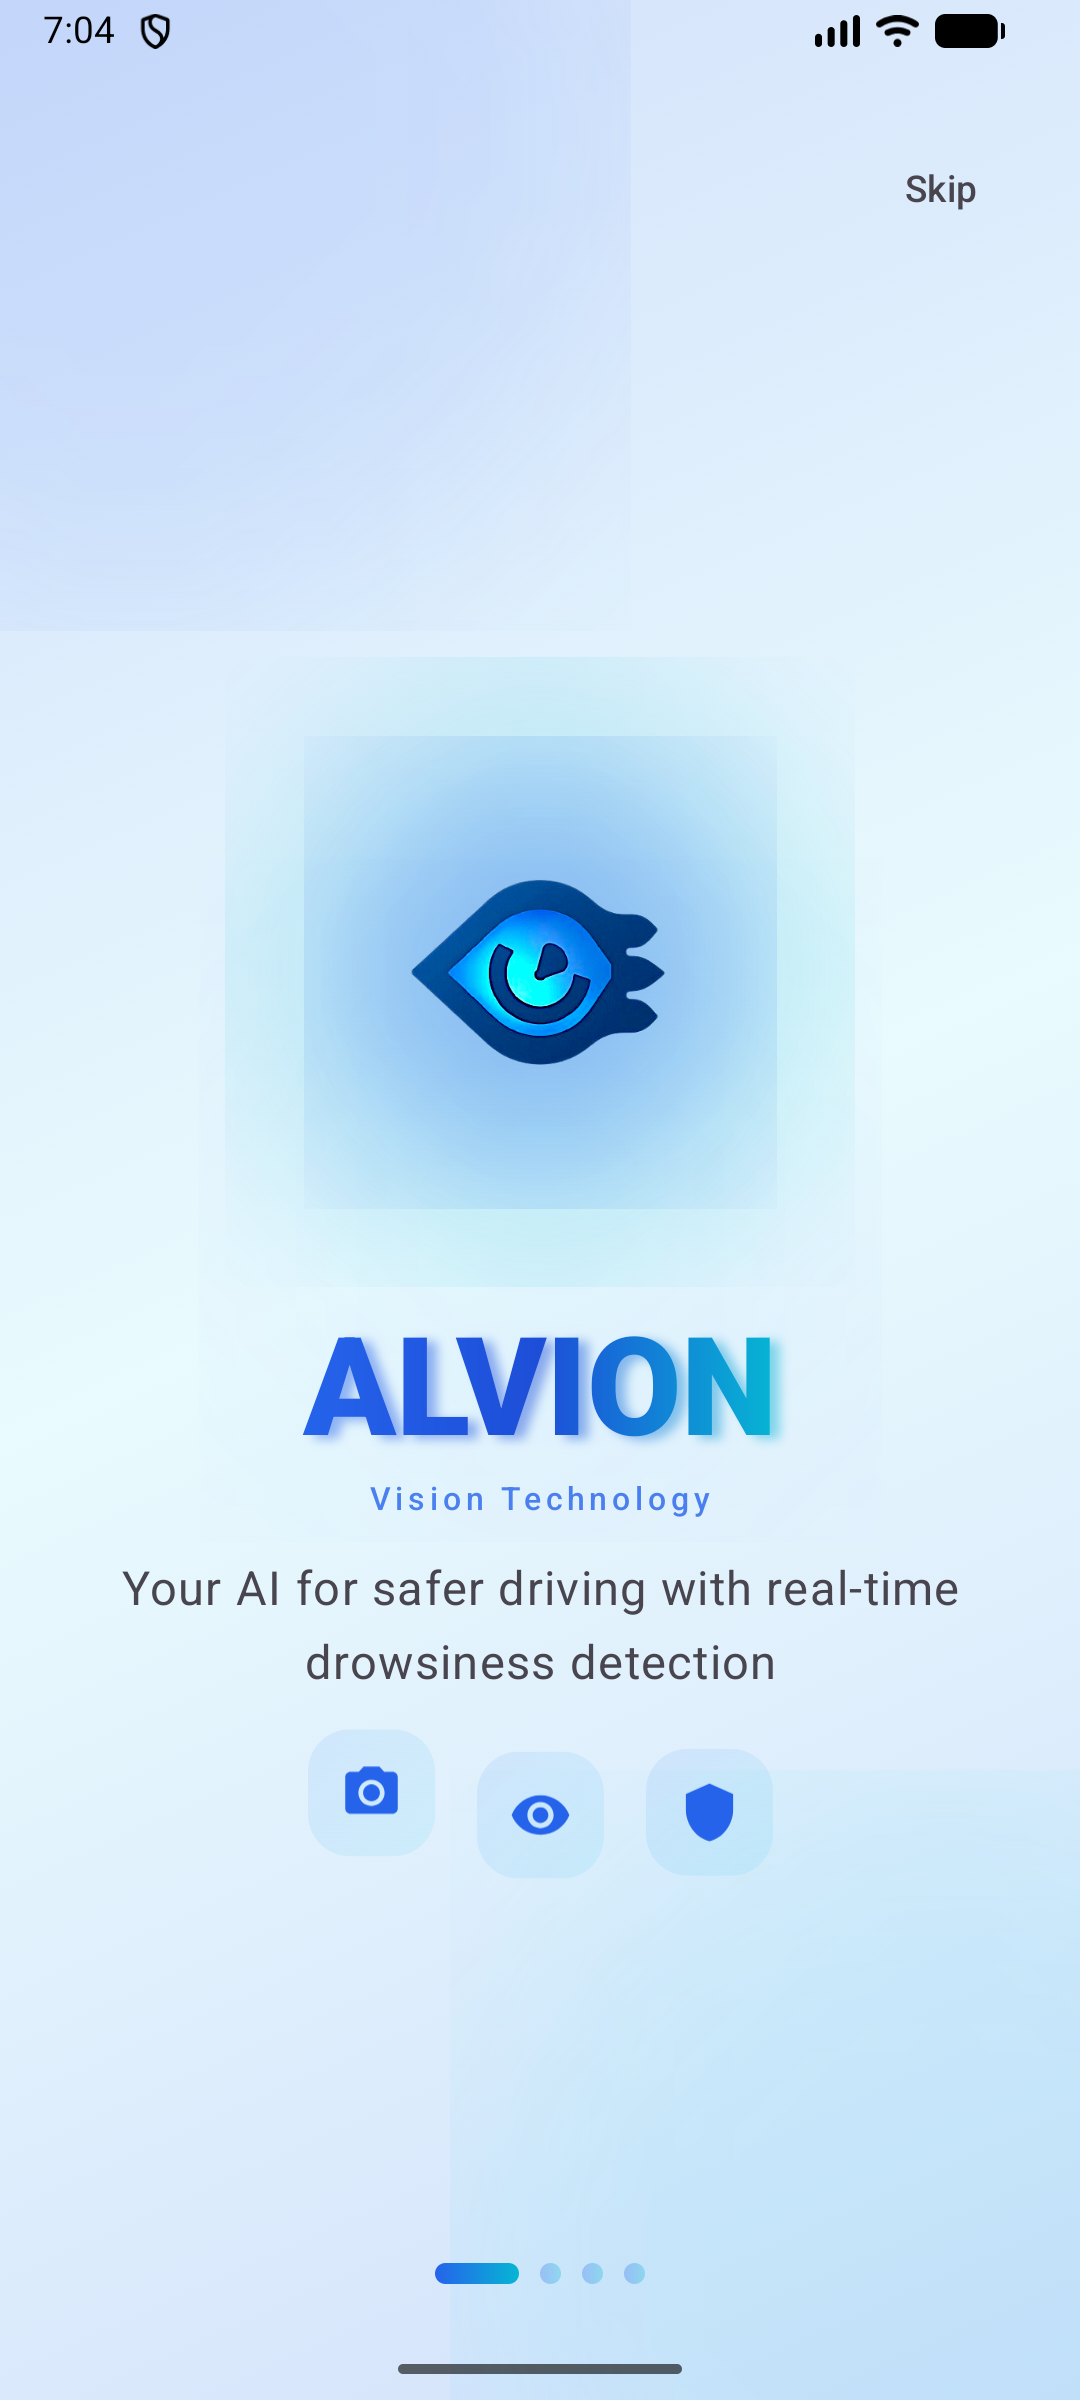
\includegraphics[width=\textwidth]{assets/UI/intro1.png}
        \caption*{Intro 1}
    \end{minipage}
    \begin{minipage}{0.24\textwidth}
        \centering
        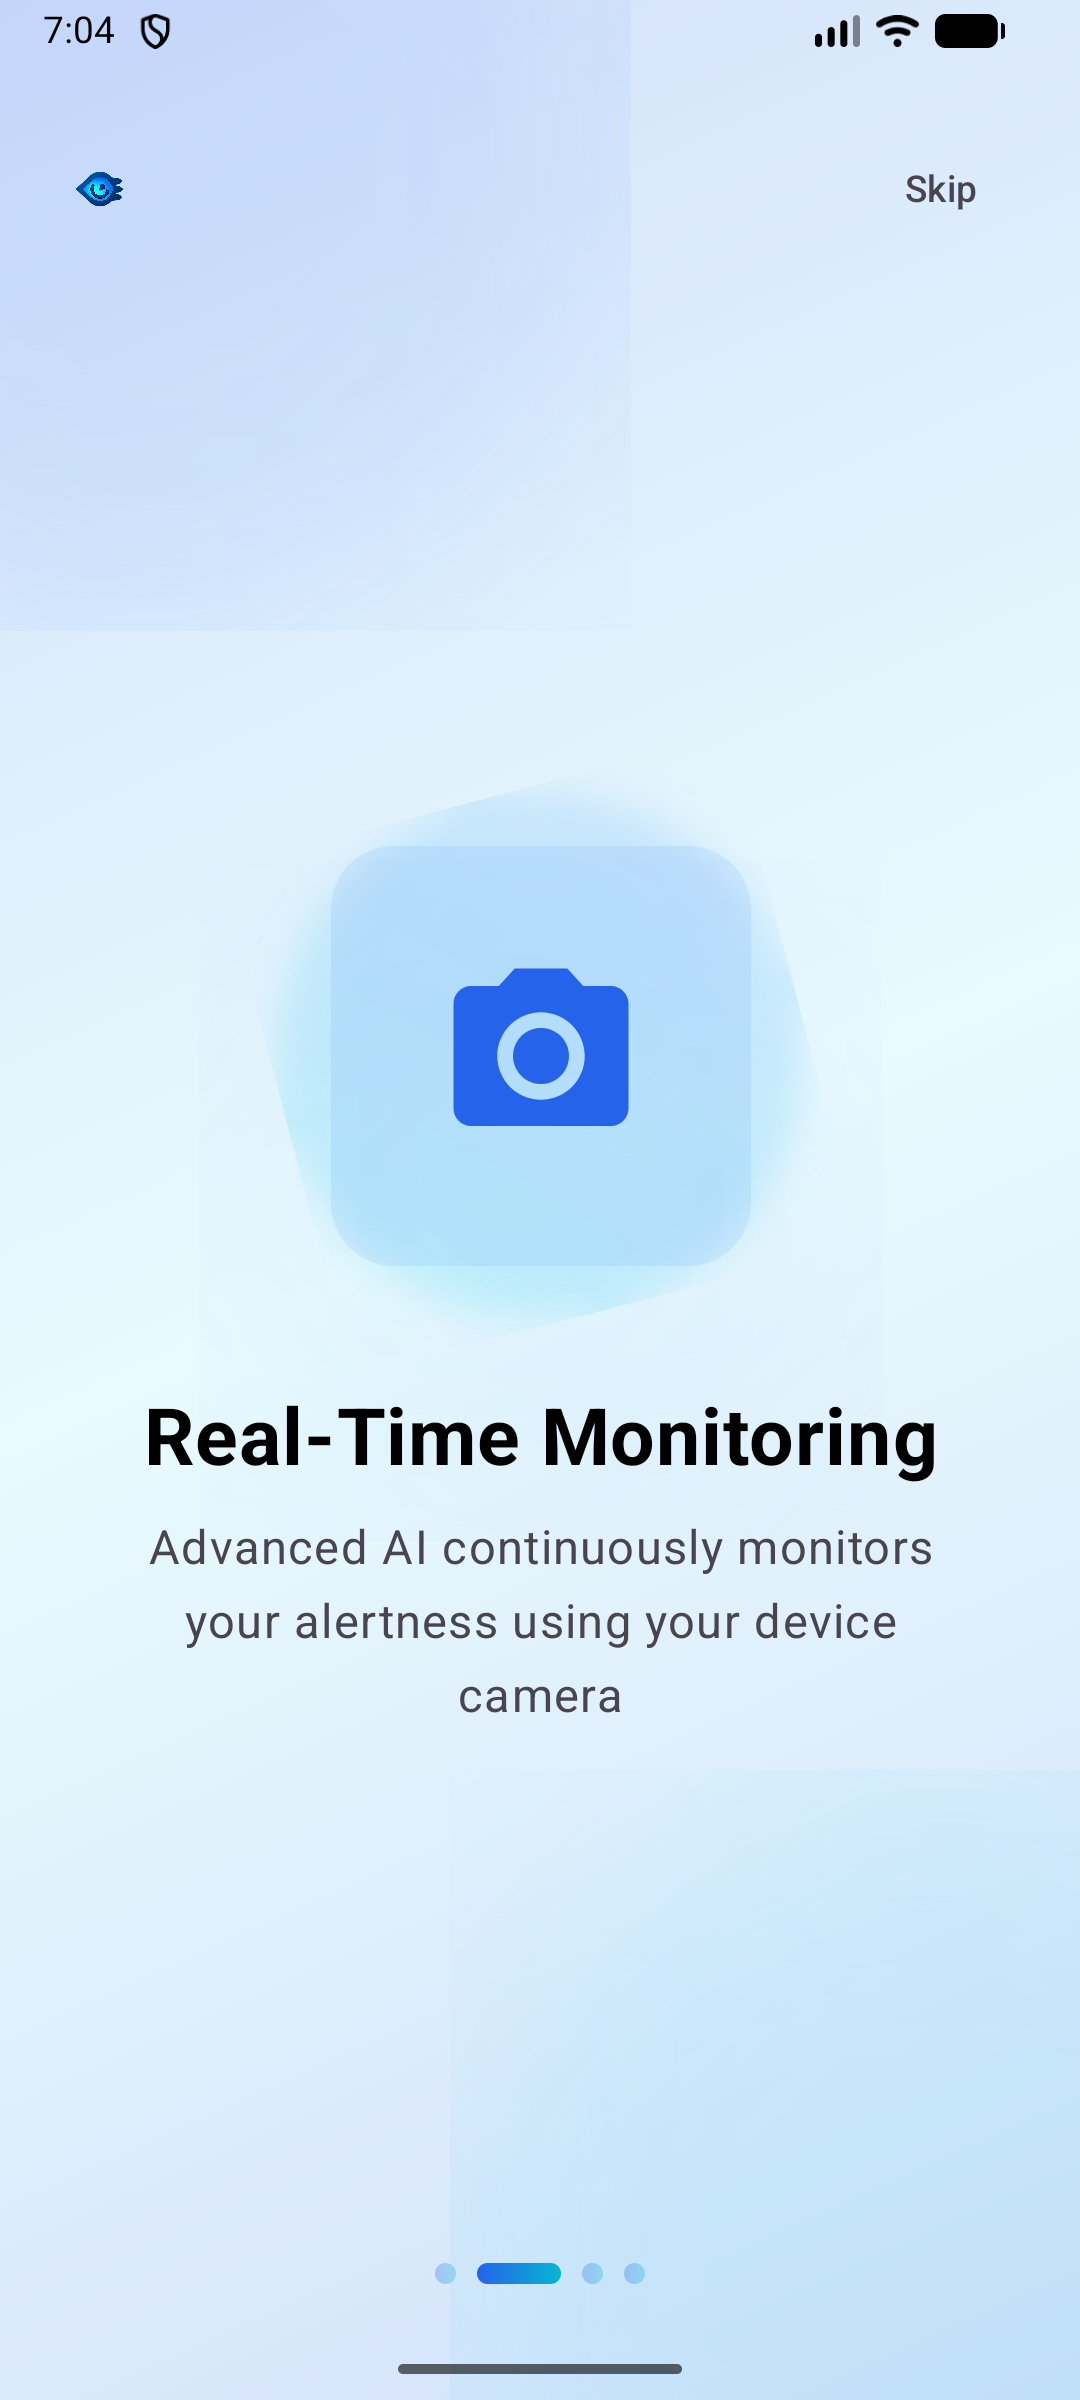
\includegraphics[width=\textwidth]{assets/UI/Intro2.png}
        \caption*{Intro 2}
    \end{minipage}
    \begin{minipage}{0.24\textwidth}
        \centering
        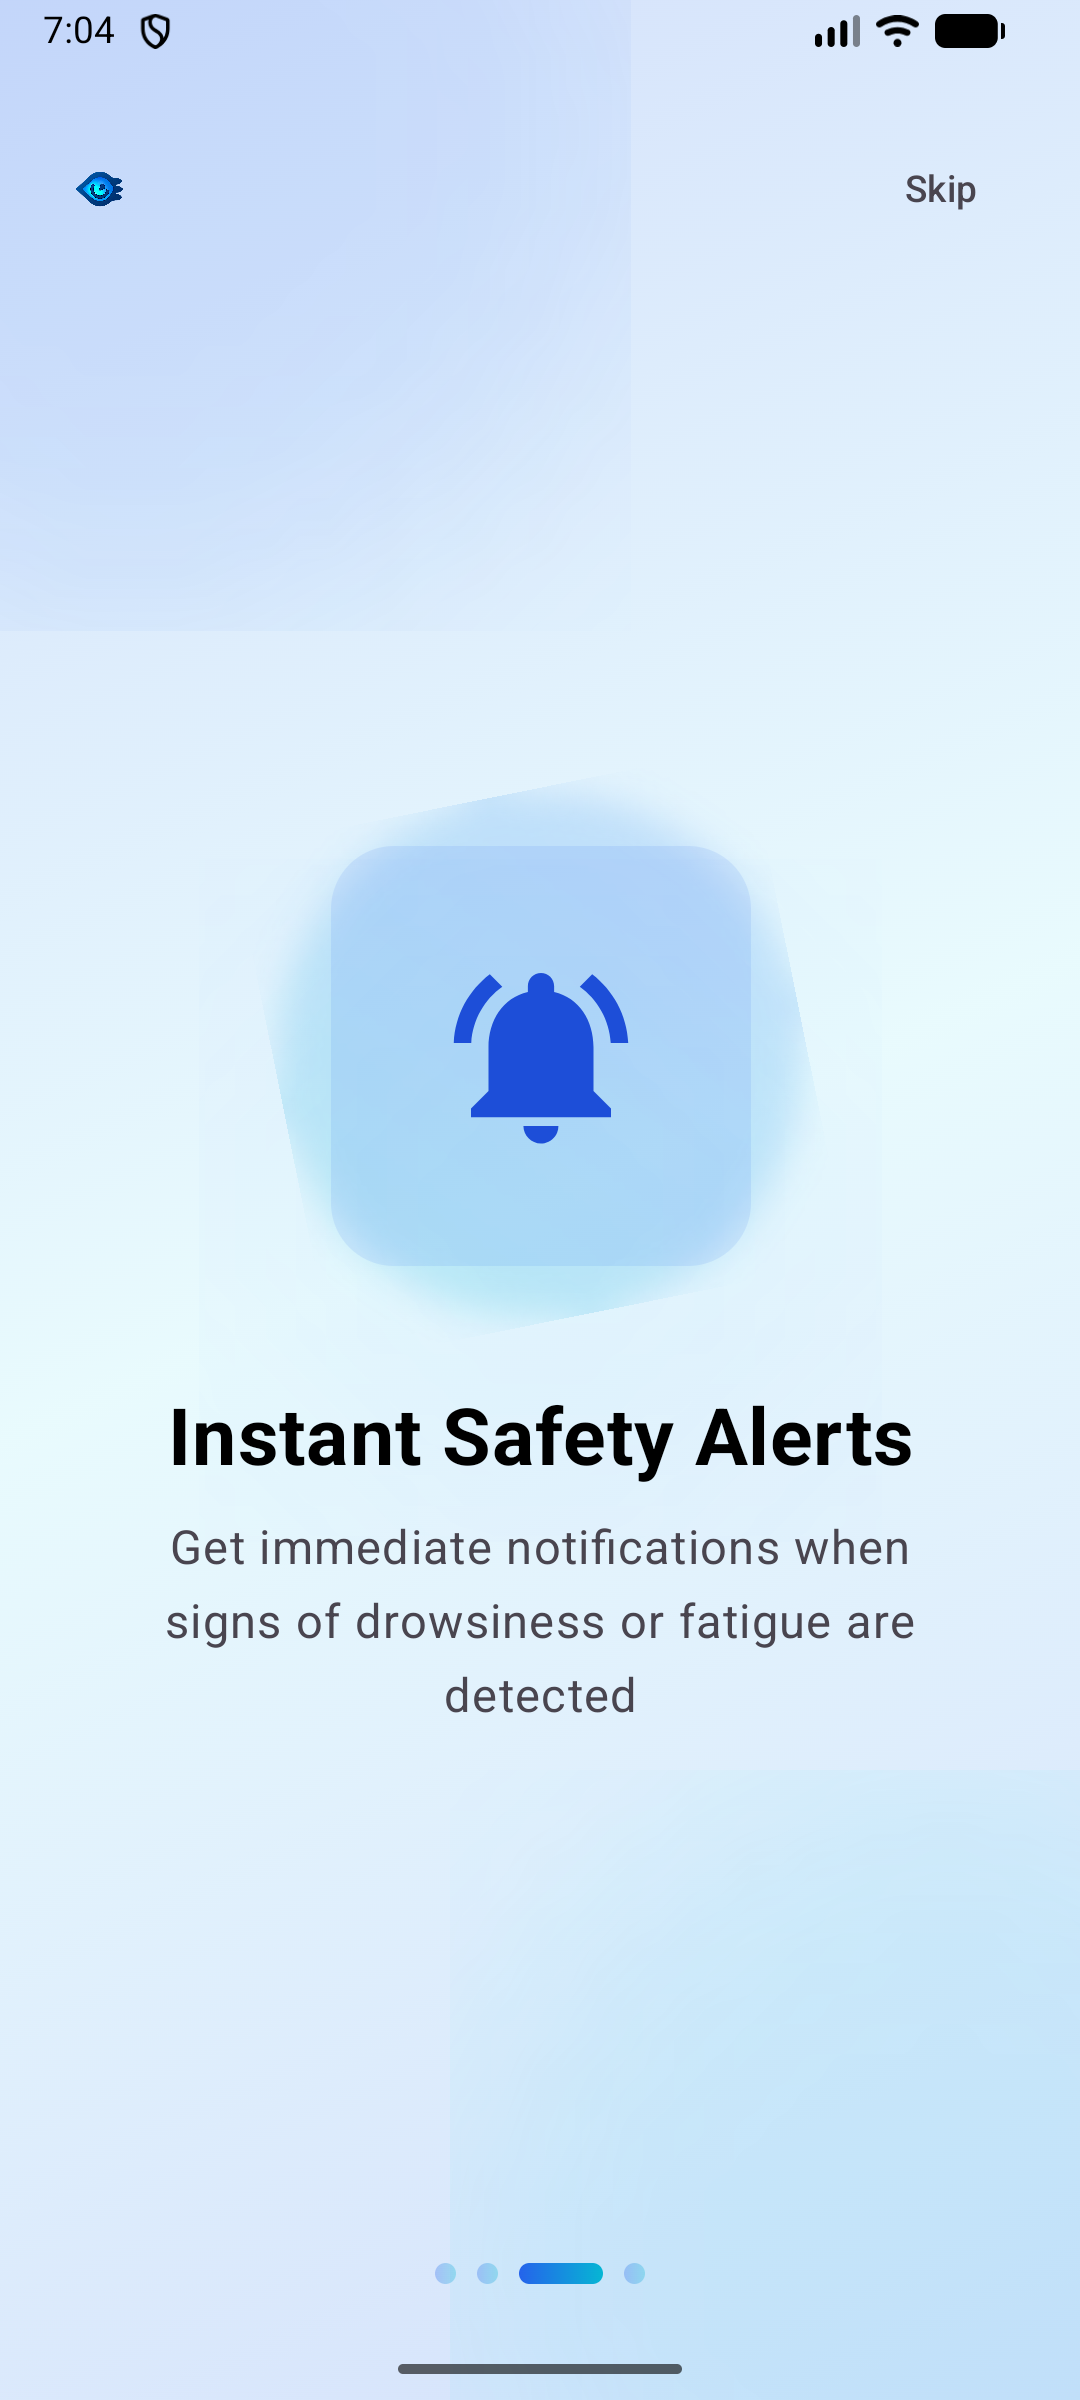
\includegraphics[width=\textwidth]{assets/UI/Intro3.png}
        \caption*{Intro 3}
    \end{minipage}
    \begin{minipage}{0.24\textwidth}
        \centering
        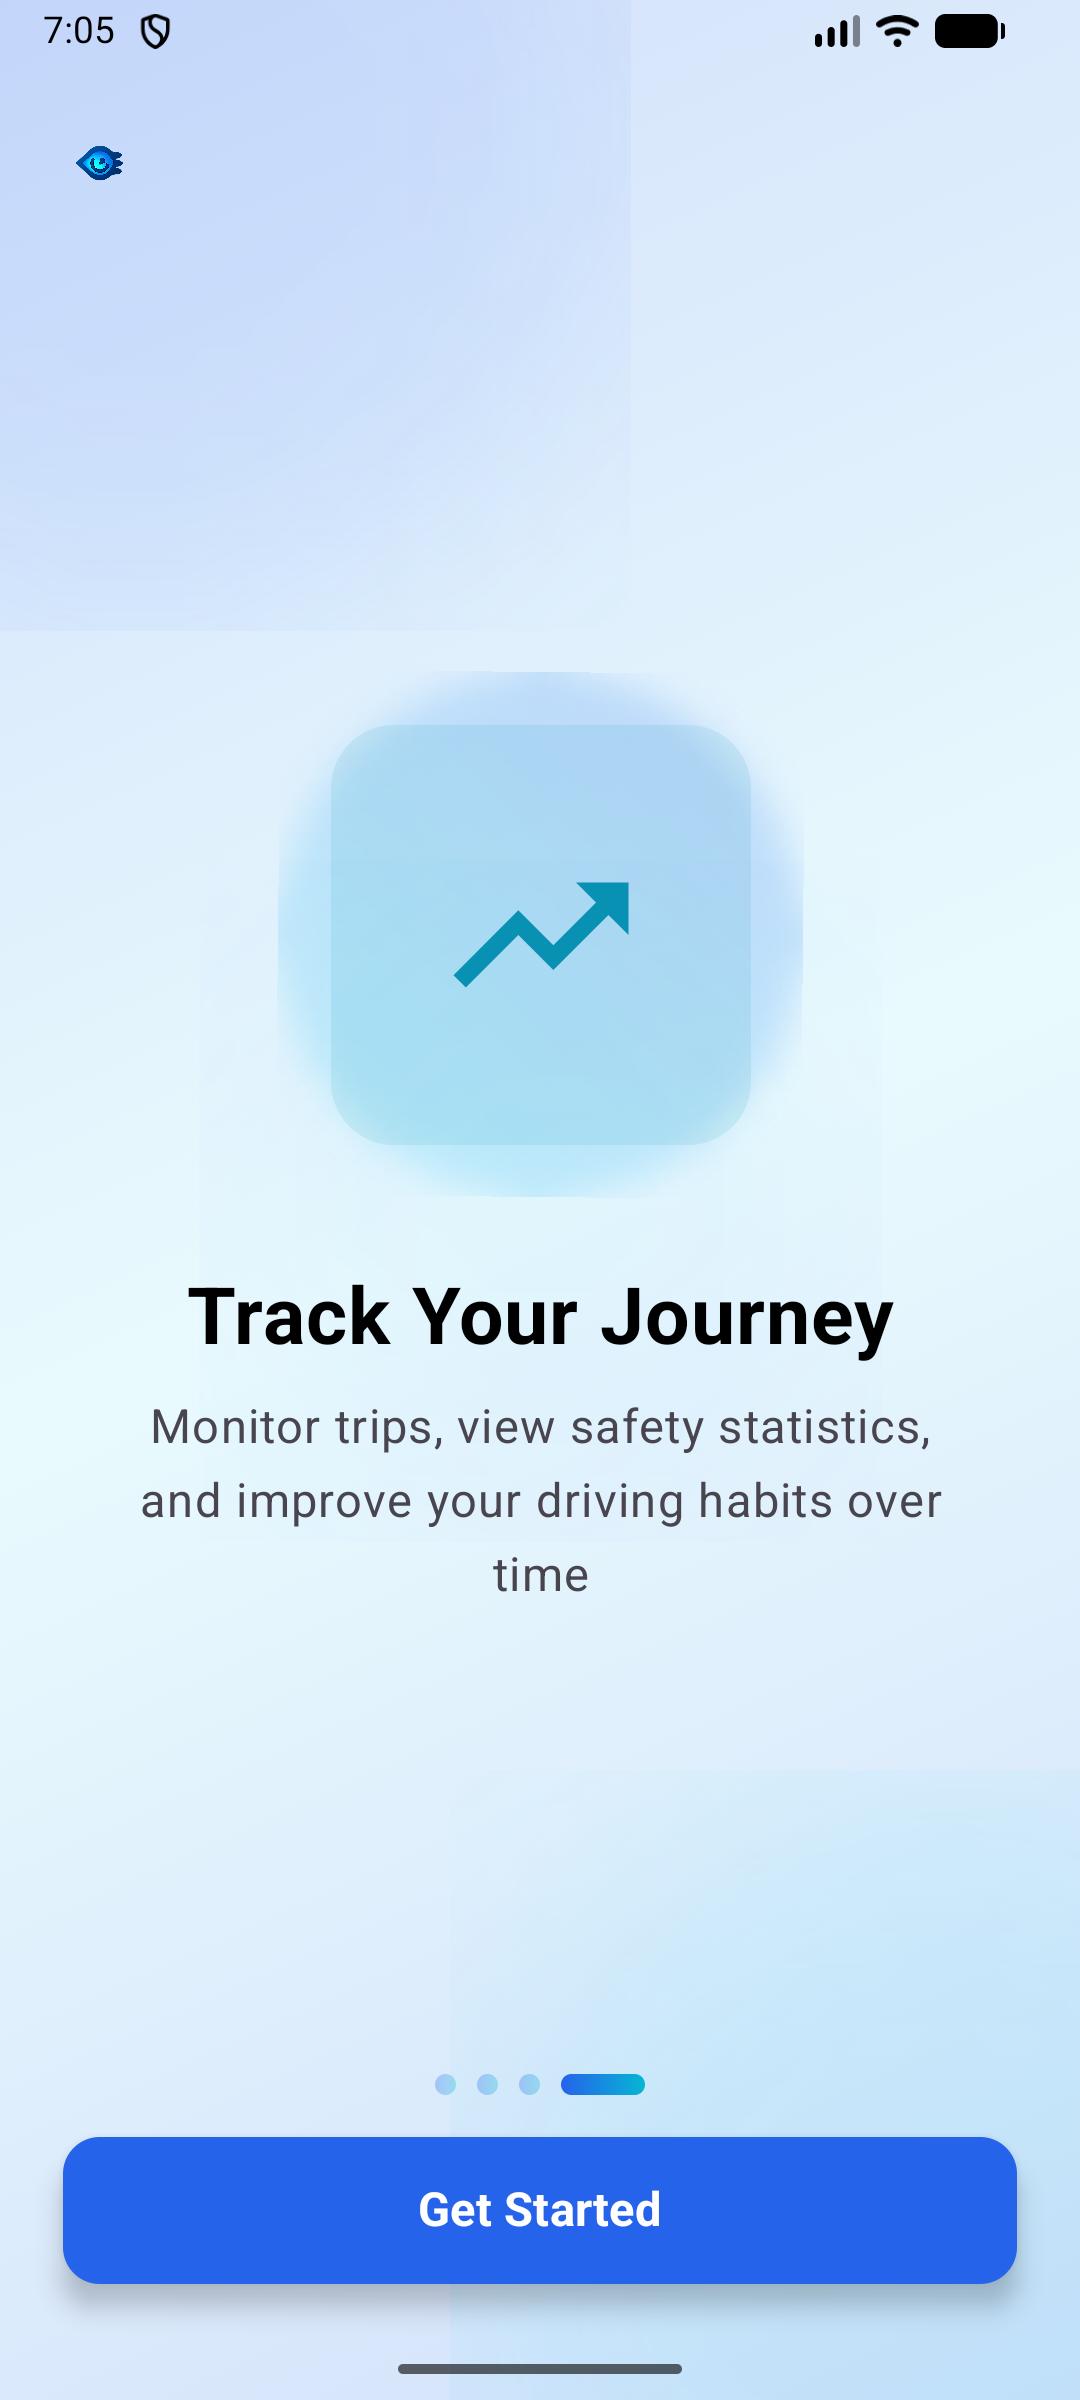
\includegraphics[width=\textwidth]{assets/UI/Intro4.png}
        \caption*{Intro 4}
    \end{minipage}
    \caption{Onboarding sequence explaining the ALVION safety features.}
\end{figure}

\begin{figure}[H]
    \centering
    \begin{minipage}{0.45\textwidth}
        \centering
        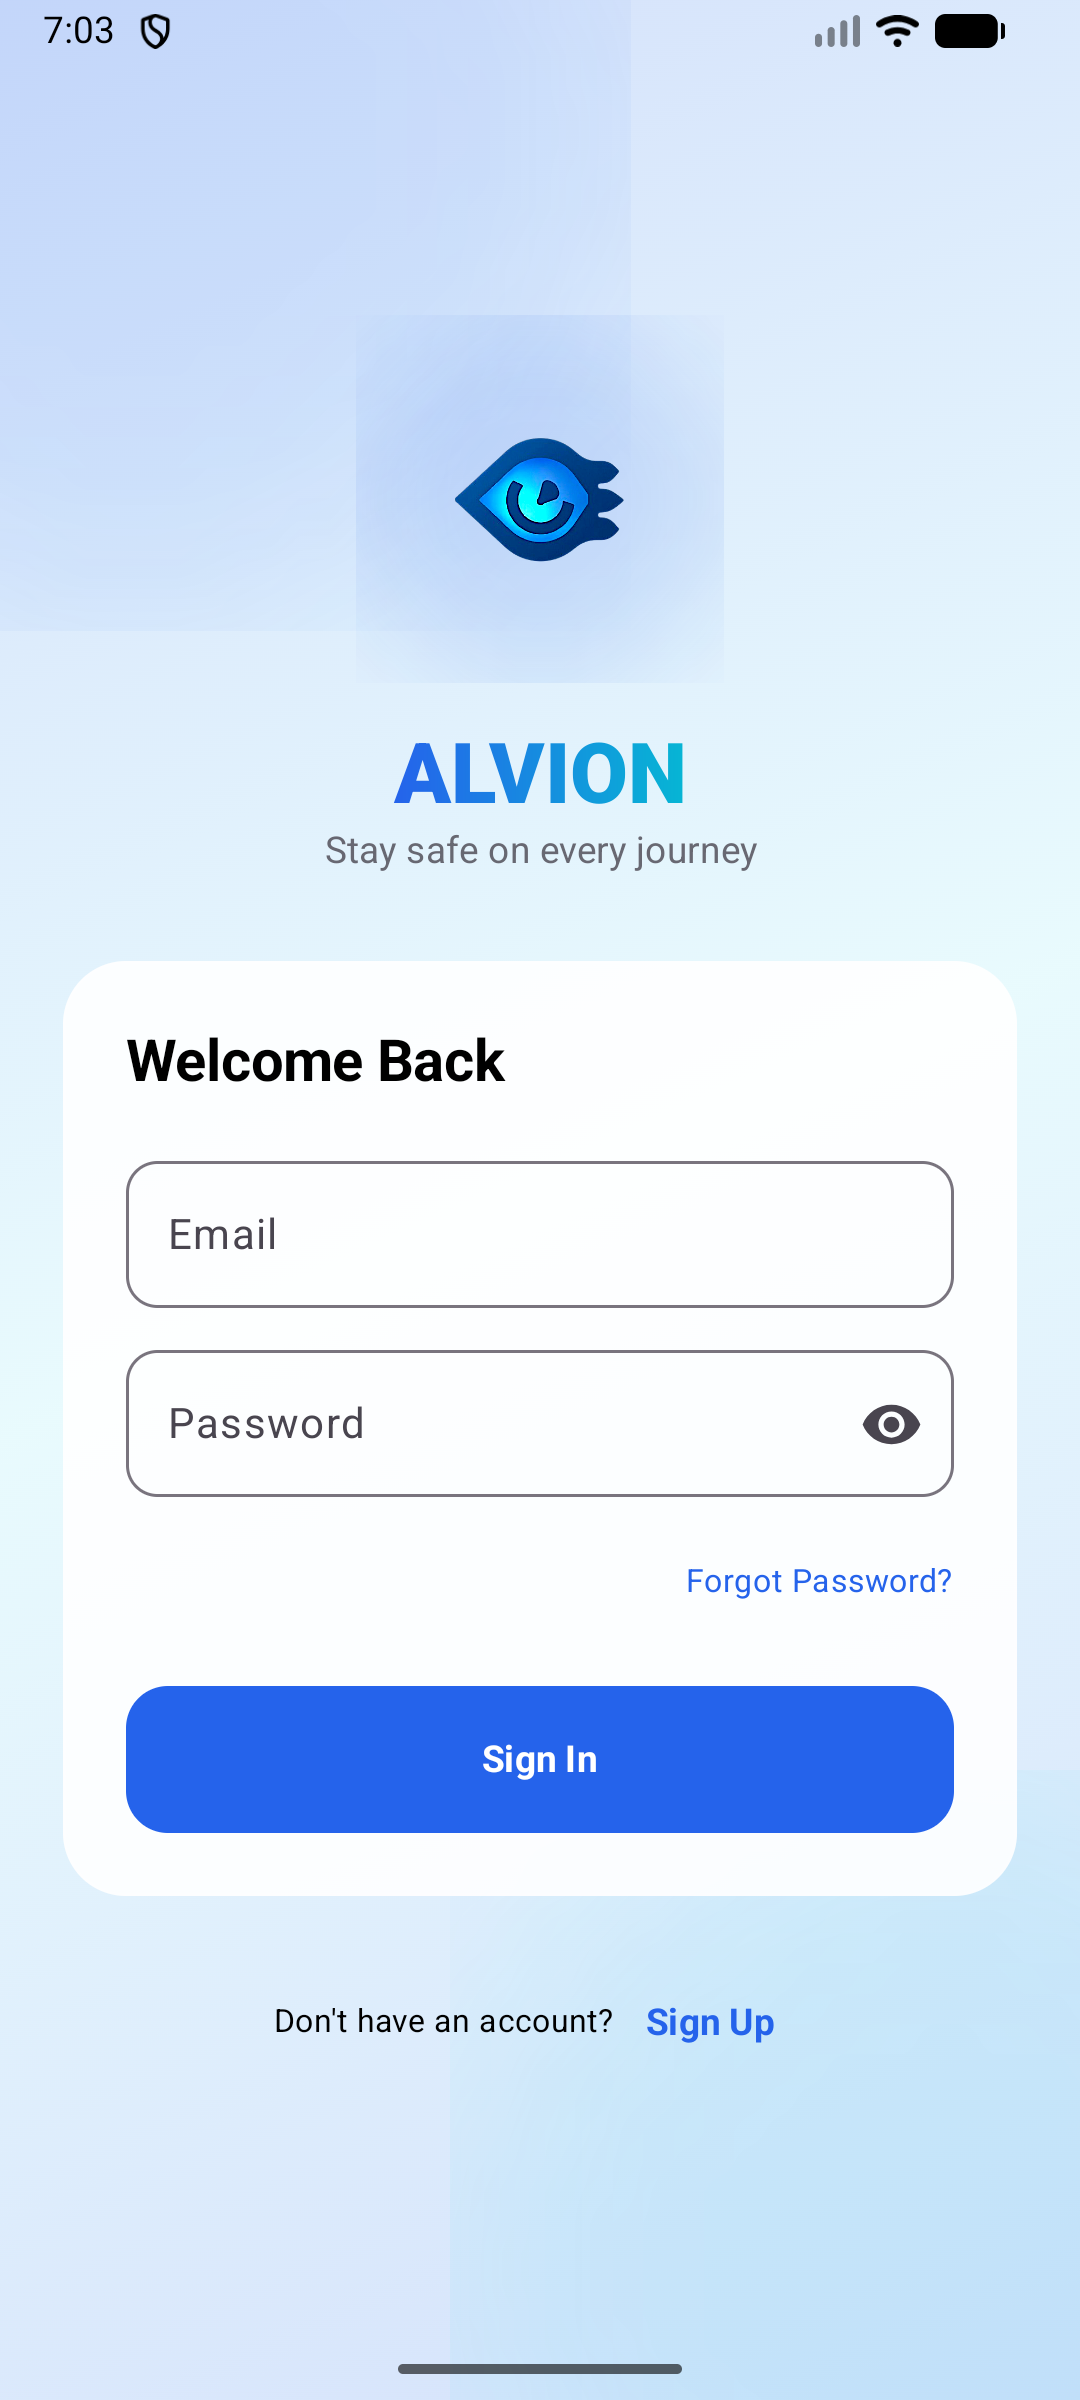
\includegraphics[width=0.7\textwidth]{assets/UI/signIn.png}
        \caption{Sign In Screen}
    \end{minipage}
    \begin{minipage}{0.45\textwidth}
        \centering
        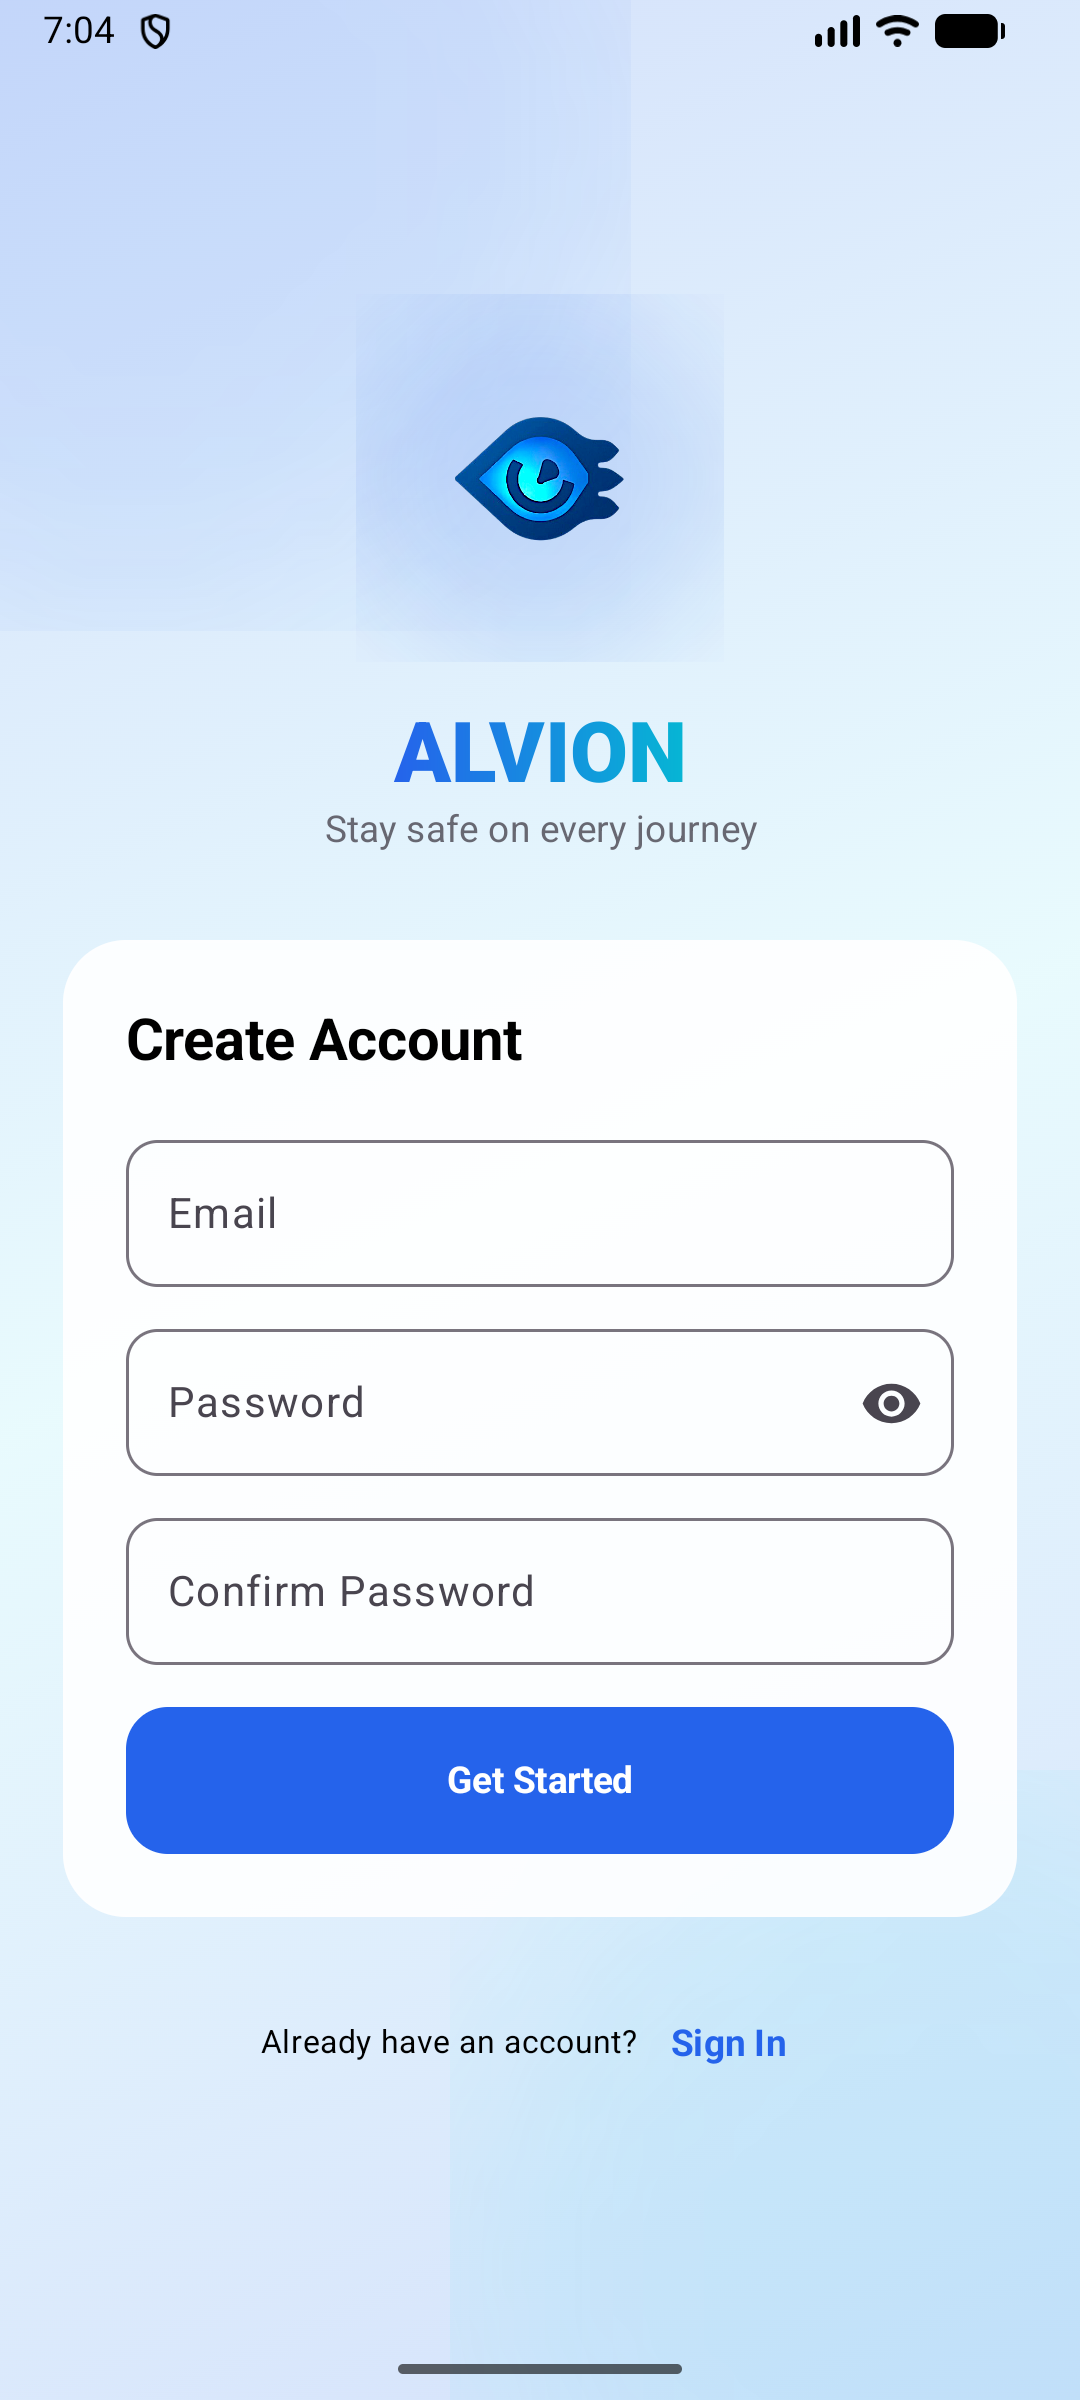
\includegraphics[width=0.7\textwidth]{assets/UI/signUp.png}
        \caption{Sign Up Screen}
    \end{minipage}
\end{figure}

\clearpage
\subsection{Main Dashboard and Monitoring}
The dashboard provides a central hub for starting sessions and managing the user profile. The monitoring screen (\textit{Face Detection}) features a minimalist overlay that prioritizes road visibility while providing real-time status cues.

\begin{figure}[H]
    \centering
    \begin{minipage}{0.32\textwidth}
        \centering
        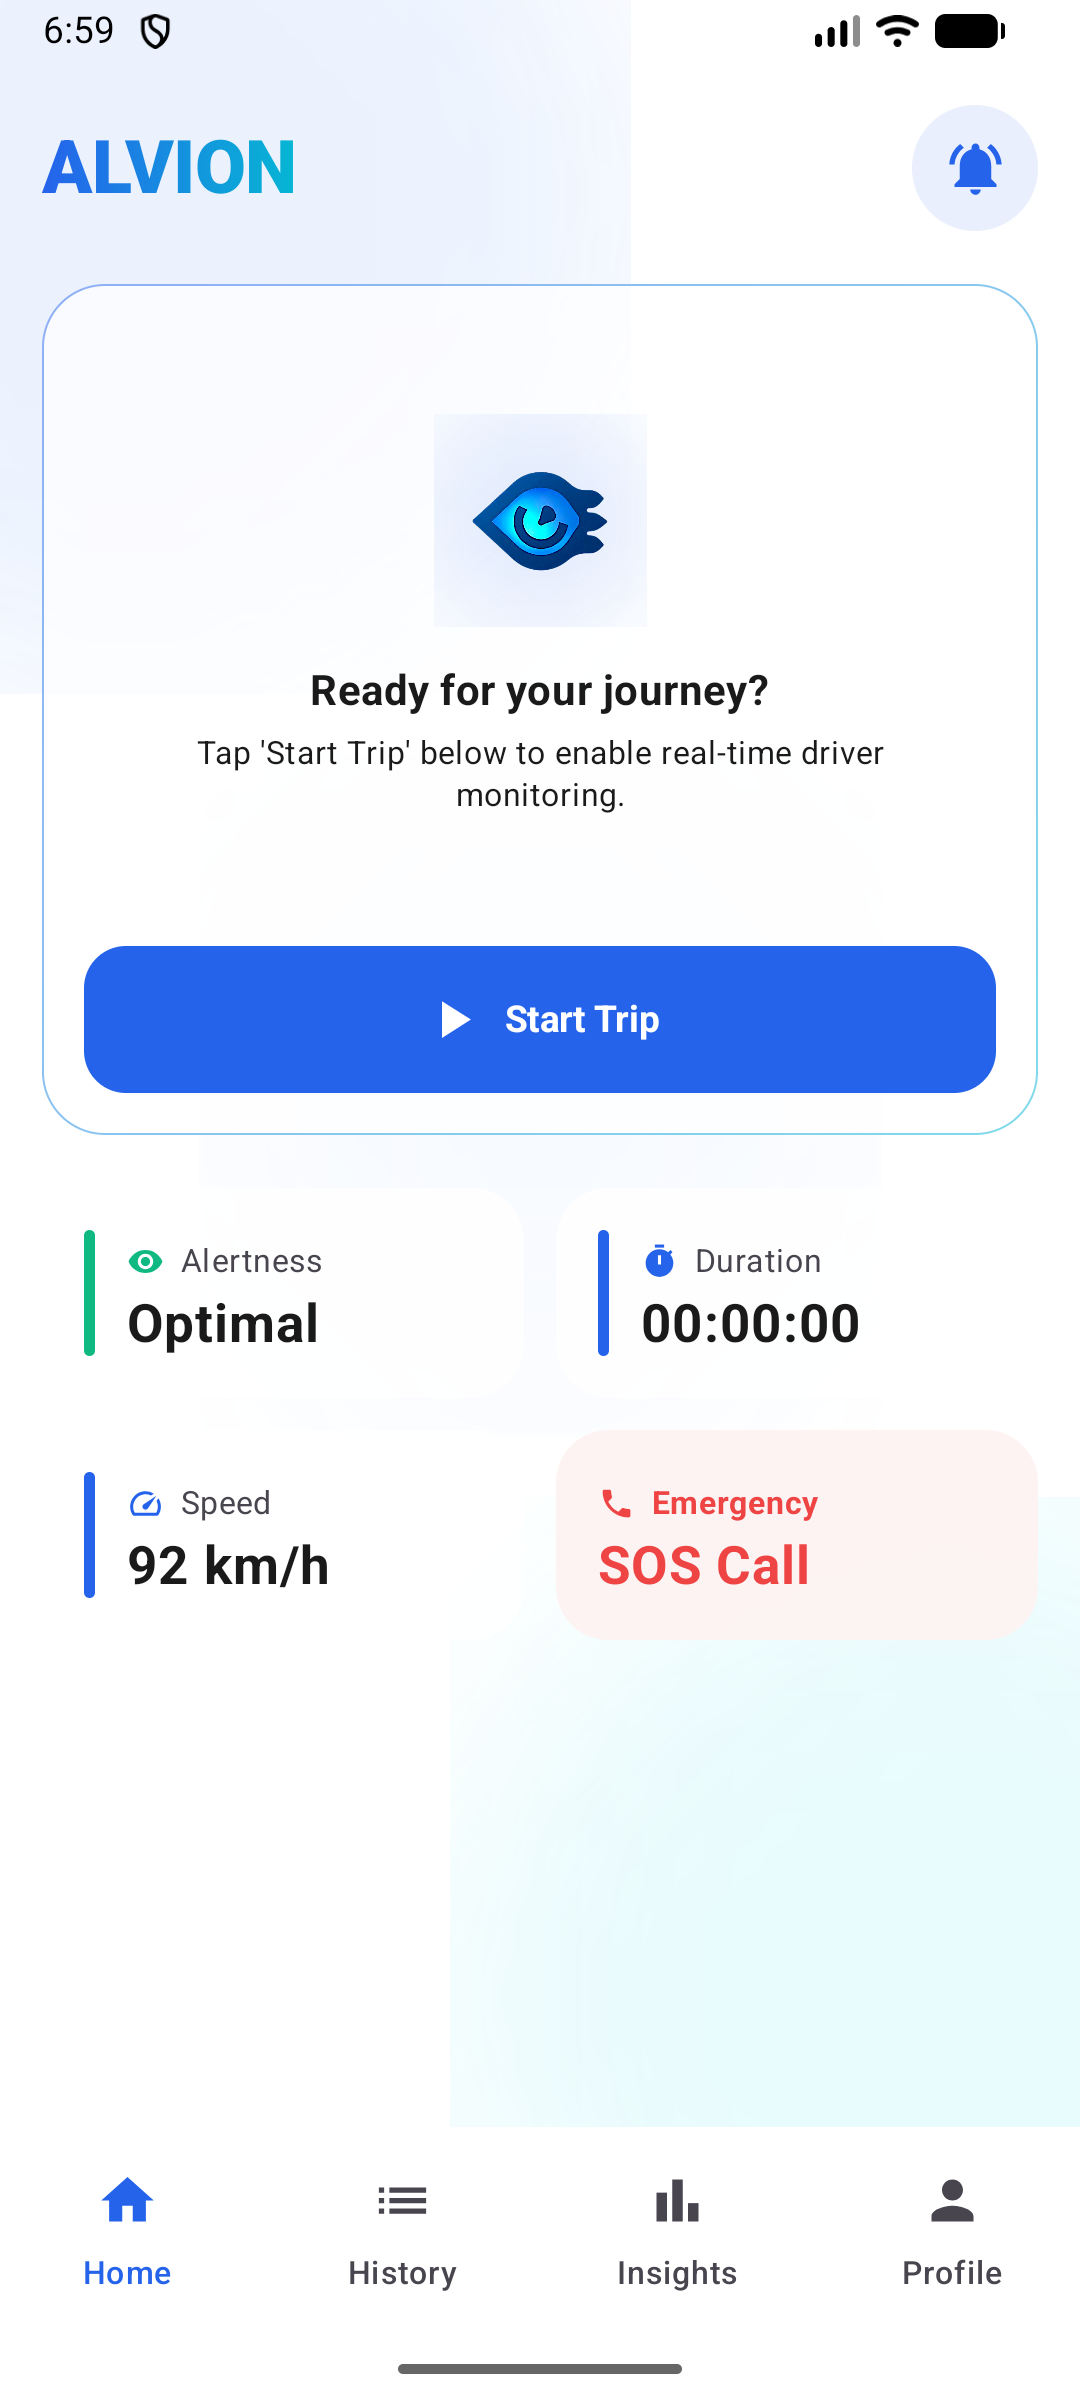
\includegraphics[width=\textwidth]{assets/UI/main.png}
        \caption{Main Dashboard}
    \end{minipage}
    \begin{minipage}{0.32\textwidth}
        \centering
        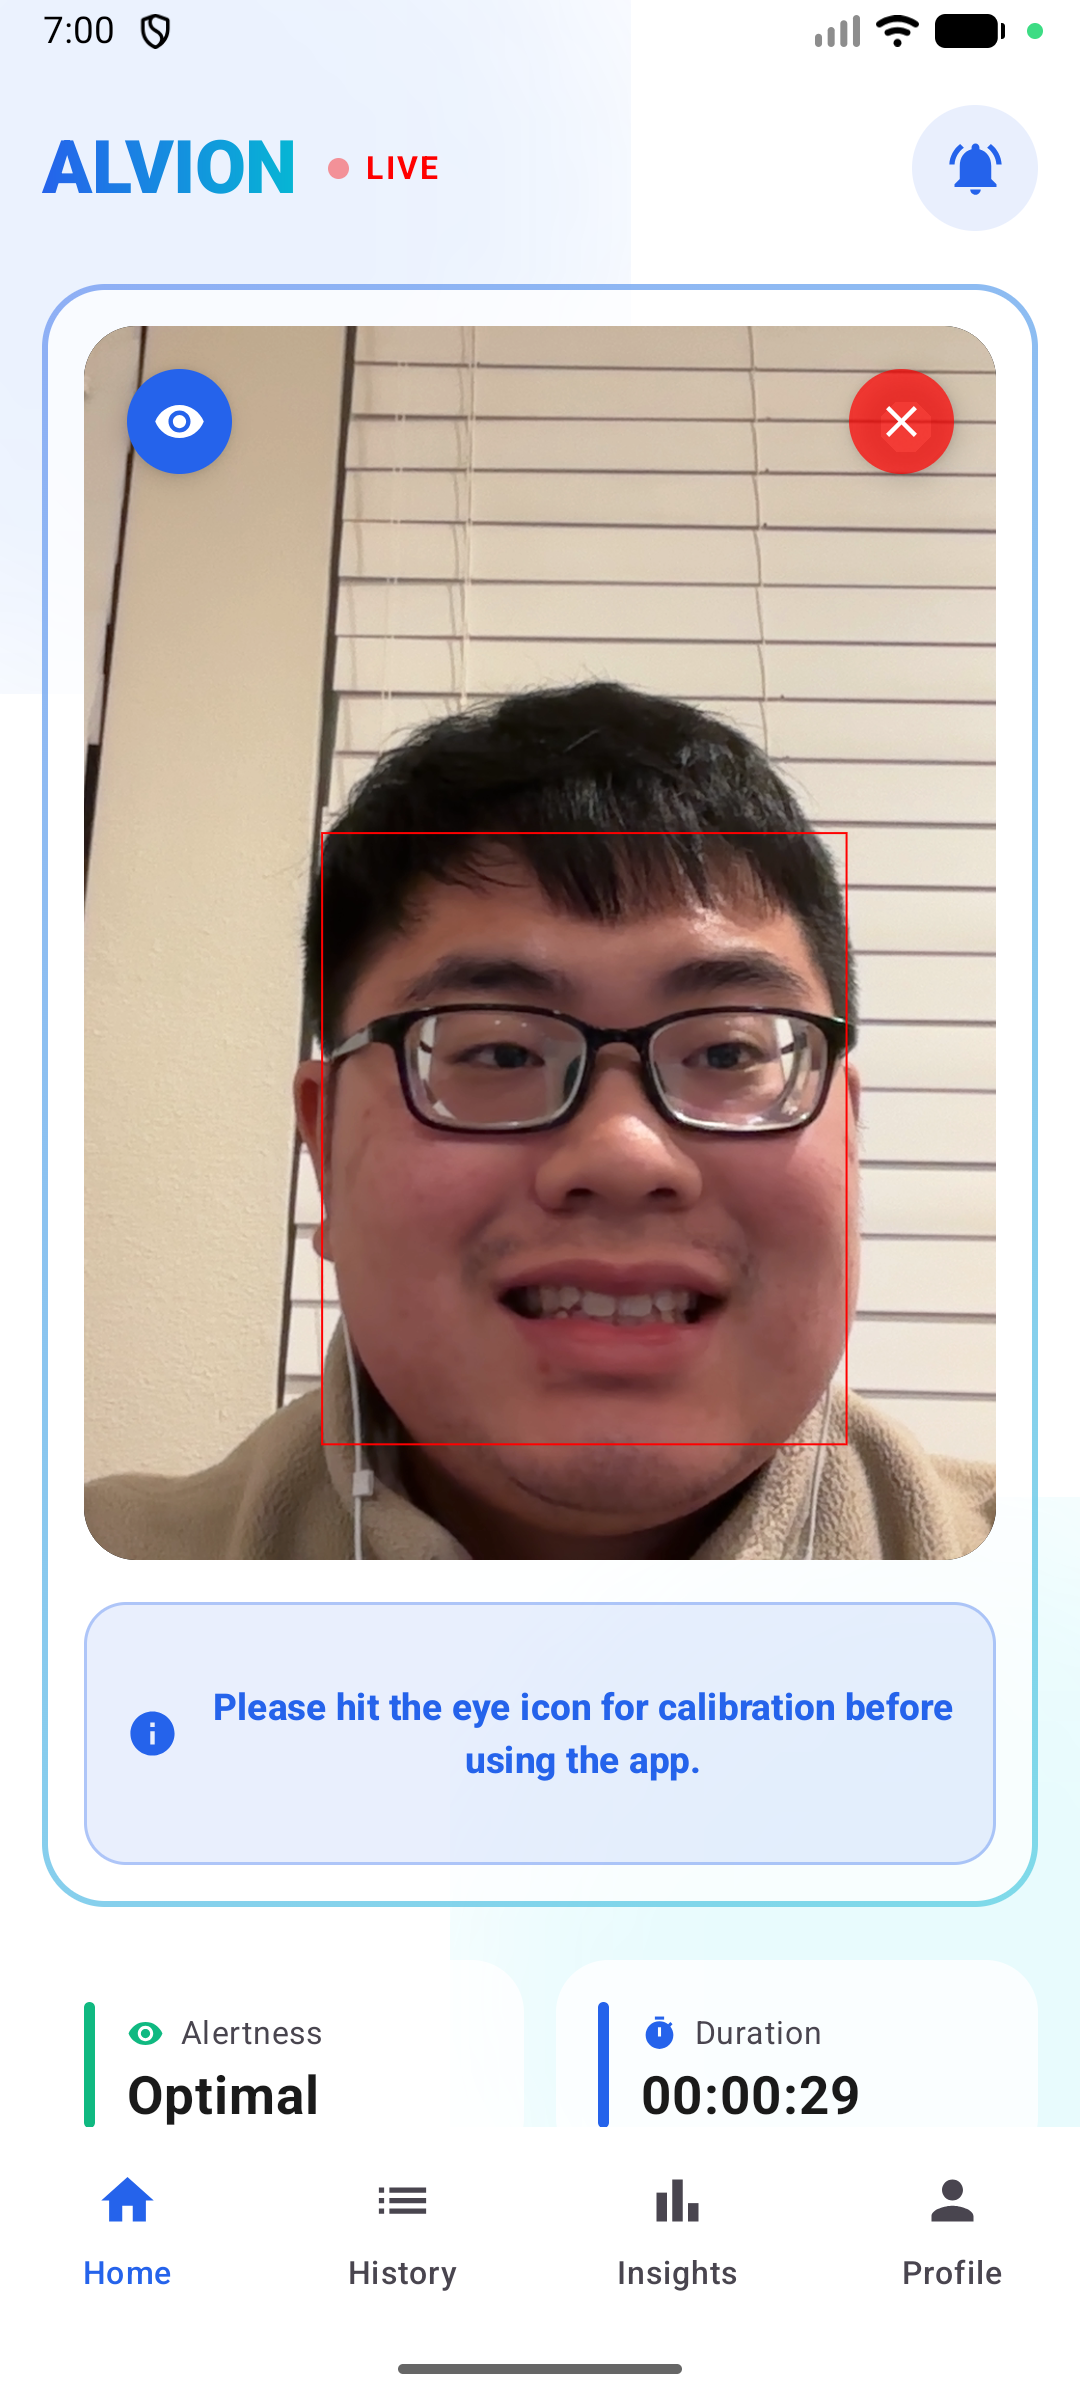
\includegraphics[width=\textwidth]{assets/UI/faceDetection.png}
        \caption{Monitoring Mode}
    \end{minipage}
    \begin{minipage}{0.32\textwidth}
        \centering
        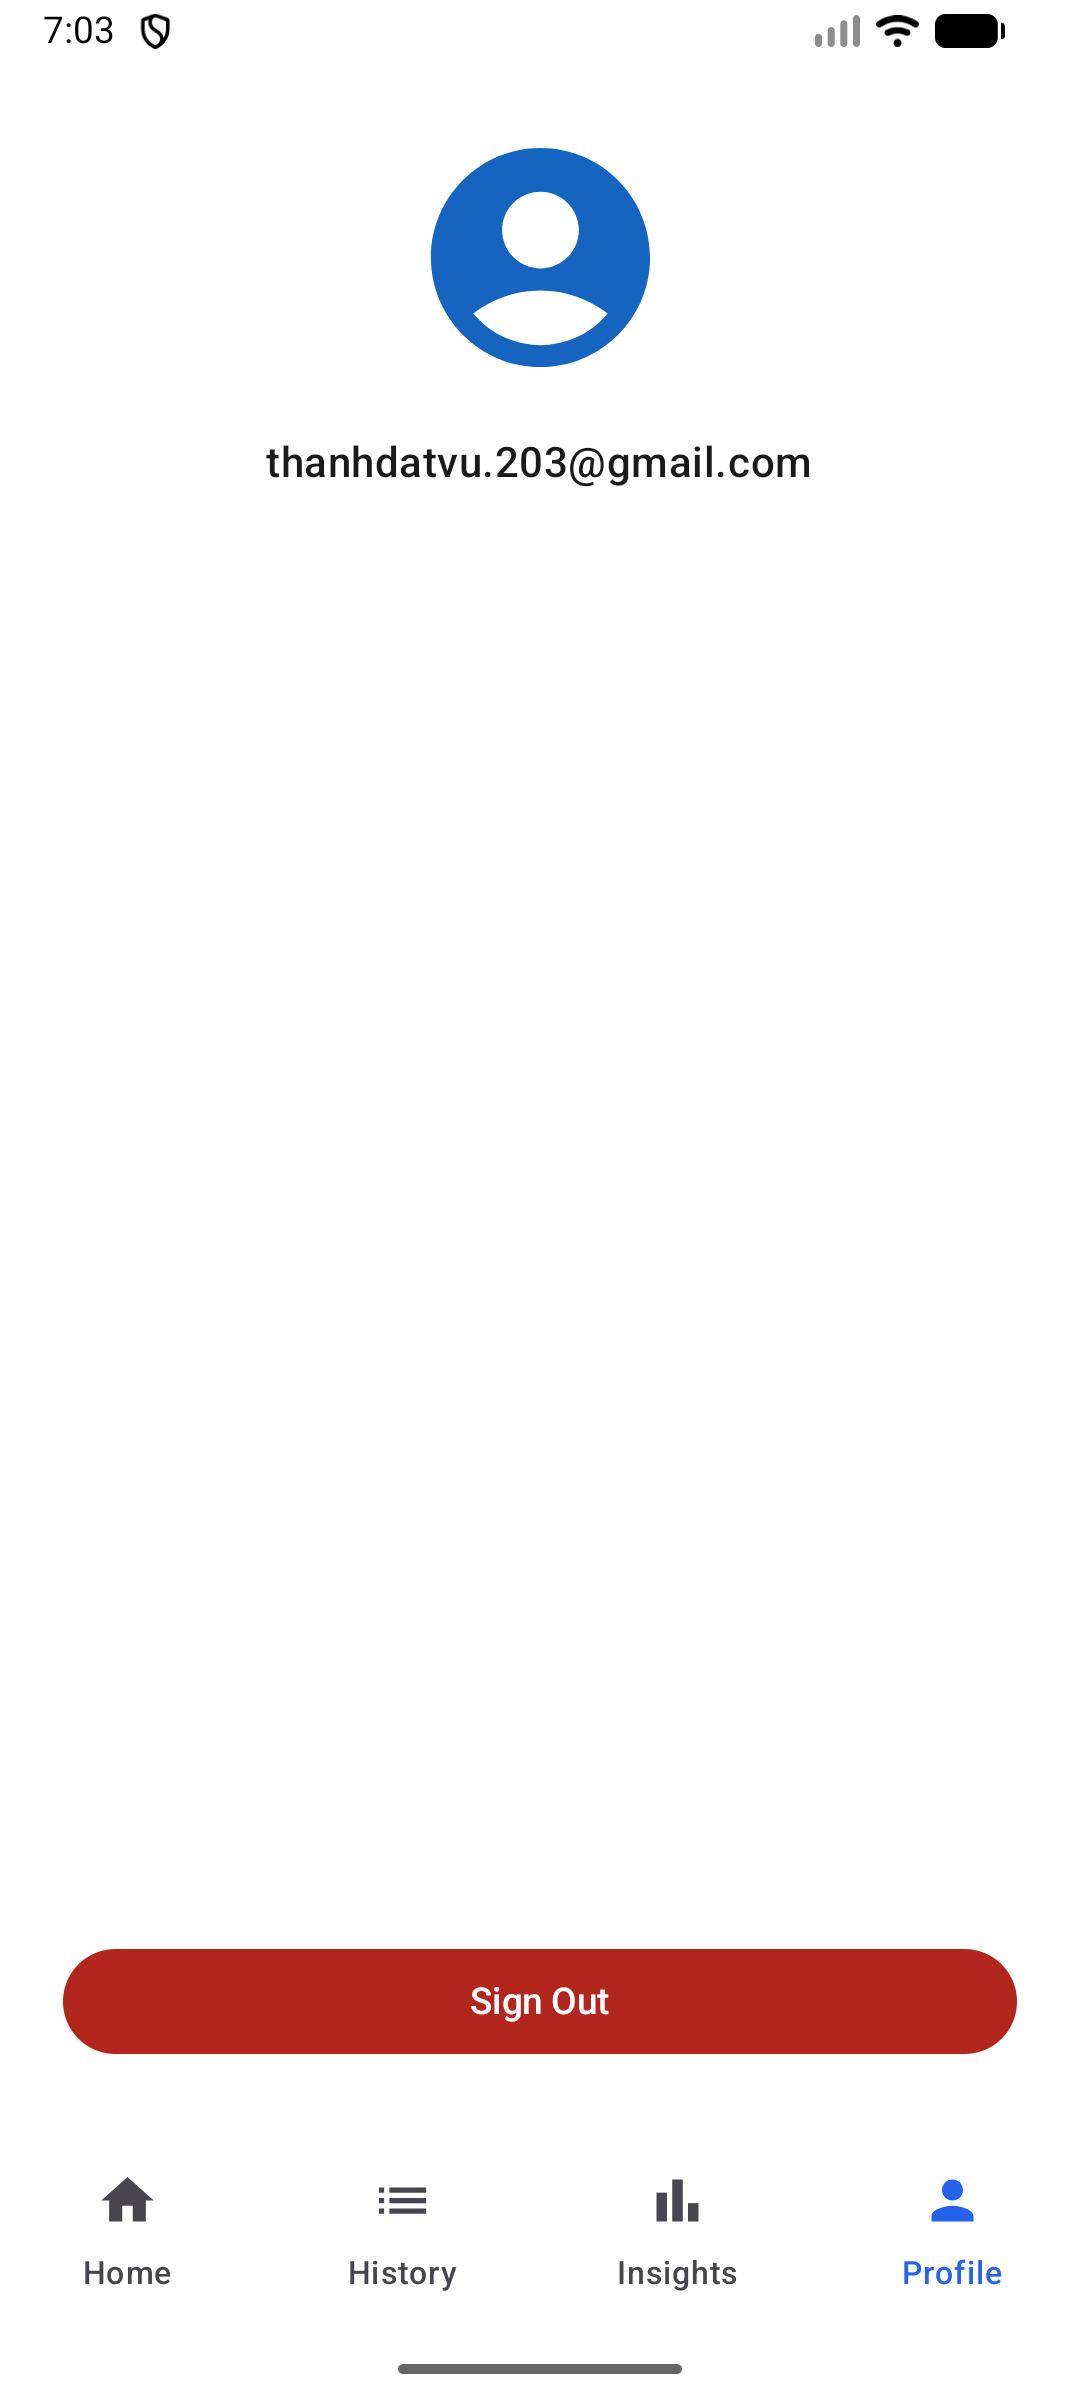
\includegraphics[width=\textwidth]{assets/UI/profile.png}
        \caption{User Profile}
    \end{minipage}
    \caption{Core application screens for monitoring and profile management.}
\end{figure}

\noindent\textbf{Design Considerations for Drivers:}
\begin{itemize}
    \item \textbf{High-Contrast Accents:} Large buttons and red alert banners are used to ensure visibility in varied cabin lighting.
    \item \textbf{Live Overlay:} The monitoring screen uses a semi-transparent graphic overlay (see \textit{GraphicOverlay.kt}) to show face tracking status without obscuring the camera preview.
    \item \textbf{Simplified Profile:} Account management is kept in a separate tab to prevent accidental interaction while the vehicle is in motion.
\end{itemize}
\clearpage

latex
% ---------- 6.4 Behavioral Design ----------
\section{Behavioral Design}\label{sec:behavioral-design}

\subsection{Sequence Diagram}\label{subsec:sequence}
\begin{figure}[H]
    \centering
    \includegraphics[width=0.9\textwidth]{assets/sequenceDiagram.png}
    \caption{Per-frame execution flow: CameraX streams frames to the \texttt{FaceDetectionAnalyzer}, which executes ML Kit inference. Resulting landmarks are evaluated by the \texttt{FaceStateEvaluator} using subjective calibration thresholds to trigger alerts.}
    \label{fig:seq-per-frame}
\end{figure}

\subsection{State Machine}\label{subsec:state-machine}
\begin{figure}[H]
    \centering
    \includegraphics[width=0.5\textwidth]{assets/statemachineDiagram.png}
    \caption{Driver State Logic: The system transitions between \textit{Normal}, \textit{Drowsy}, and \textit{Distracted} states. Transitions are gated by dwell timers (e.g., $1,800$~ms for eyes) and yaw hysteresis to prevent oscillating alerts.}
    \label{fig:state-driver}
\end{figure}

\begin{figure}[H]
    \centering
    \includegraphics[width=0.4\textwidth]{assets/activityDiagram.png}
    \caption{User Configuration Flow: Settings updates are persisted to \texttt{SharedPreferences}. The \texttt{FaceStateEvaluator} observes these changes to dynamically update sensitivity thresholds without restarting the monitoring session.}
    \label{fig:activity-settings}
\end{figure}

% ---------- 6.5 Design Alternatives \& Decision Rationale ----------
\section{Design Alternatives \& Decision Rationale}\label{sec:design-alternatives}

\noindent\textbf{On-device vs. Cloud.}
We prioritized on-device inference using the ML Kit SDK to ensure sub-200ms latency and to preserve driver privacy. Cloud-based processing was rejected due to its dependency on network stability and the security risks associated with transmitting raw facial video data.

\vspace{1em}
\noindent\textbf{Landmark Rules vs. End-to-End Classifiers.}
The system utilizes a heuristic "rules-based" approach (PERCLOS and Yaw Delta) rather than an end-to-end deep learning model (e.g., a "Drowsy vs. Alert" binary classifier). This decision was made to allow for \textbf{subjective calibration}. By using landmarks, we can establish a unique "Forward" baseline for each driver, which is more robust than a generic model that might struggle with different seating positions or mounting angles.

\vspace{1em}
\noindent\textbf{ML Kit vs. Custom Model Training.}
We chose the pre-trained ML Kit Face Detection API over training a custom CNN. ML Kit is highly optimized for Android's Neural Networks API (NNAPI) and provides reliable eye-openness and Euler angle metrics out of the box. This allowed the development team to focus on the complex safety logic—such as Mirror Symmetry and EMA smoothing—rather than the low-level vision tasks.

\vspace{1em}
\noindent\textbf{Volatile Frame Analysis.}
A key design decision was to implement "volatile" processing. The \texttt{FaceDetectionAnalyzer} processes frames in-memory and immediately closes the \texttt{ImageProxy} once landmarks are extracted. This ensures that no image data is ever written to disk, satisfying the project's strict privacy requirements and reducing storage overhead.

\vspace{1em}
\noindent\textbf{Temporal Smoothing (EMA).}
To mitigate sensor noise from ML Kit, we implemented an Exponential Moving Average (EMA) for eye-openness scores. This alternative was chosen over a simple moving average to give more weight to recent frames, allowing for a faster response to sudden eyelid closure while still filtering out momentary blinks that could cause false drowsiness alerts.

\clearpage

% ========================= 7. SYSTEM IMPLEMENTATION =========================
\chapter{System Implementation}\label{ch:system-implementation}

% ---------- 7.1 Programming Languages \& Tools ----------
\section{Programming Languages \& Tools}\label{sec:prog-tools}

Our prototype is built using a modern Android stack, prioritizing on-device performance and maintainable code.

\begin{itemize}
    \item \textbf{Android Studio \& Kotlin:} The primary development environment and language. We utilize Kotlin's high-order functions for event callbacks (\texttt{onDrowsy}, \texttt{onDistracted}).
    \item \textbf{Jetpack Compose:} Used for the entire UI layer, including the \texttt{GraphicOverlay} that renders real-time tracking feedback.
    \item \textbf{CameraX (ImageAnalysis):} Provides the \texttt{Analysis} stream. We implement the \texttt{ImageAnalysis.Analyzer} interface to process frames asynchronously.
    \item \textbf{ML Kit Face Detection:} Our core vision engine. It is configured in \texttt{PERFORMANCE\_MODE\_ACCURATE} to ensure reliable eye-openness and Euler angle extraction.
    \item \textbf{Firebase Authentication:} Handles user identity and secure access to the application's monitoring features.
\end{itemize}

% ---------- 7.2 Coding Conventions ----------
\section{Coding Conventions}\label{sec:coding-conventions}
The project follows standard Android/Kotlin guidelines with a focus on \textbf{Clean Architecture} principles:

\begin{itemize}
    \item \textbf{Separation of Concerns:} Logic is strictly separated into \texttt{util} (math/logic), \texttt{components} (UI widgets), and \texttt{feature} (screen-level state).
    \item \textbf{Immutability:} We prioritize \texttt{val} and immutable state models to prevent side effects in the vision pipeline.
    \item \textbf{Interface-Driven Design:} Core components like the \texttt{FaceProcessor} and \texttt{MainThreadPoster} are abstracted behind interfaces to facilitate unit testing.
\end{itemize}

% ---------- 7.3 Code Version Control ----------
\section{Code Version Control}\label{sec:version-control}
\begin{itemize}
    \item \textbf{GitHub Hosting:} The repository is hosted on GitHub, using a branch-per-feature strategy.
    \item \textbf{Atomic Commits:} We ensure each commit represents a single, testable change to the system.
    \item \textbf{CI/CD Integration:} GitHub Actions are used to run automated lint checks and unit tests (e.g., \texttt{FaceLogicTest.kt}) on every pull request.
\end{itemize}

% ---------- 7.4 Implementation Alternatives \& Decision Rationale ----------
\section{Implementation Alternatives \& Decision Rationale}\label{sec:impl-alternatives}

\begin{itemize}
    \item \textbf{Inference Strategy:} We chose \textbf{ML Kit} over custom TFLite models. This decision significantly reduced the APK size and eliminated the need for manual HWC (Hardware Configuration) mapping, as ML Kit automatically utilizes the Snapdragon NPU/GPU via NNAPI.
    \item \textbf{Threading Model:} We use an \texttt{AndroidMainThreadPoster} interface to delegate UI updates. This ensures that the heavy mathematical evaluation in \texttt{FaceStateEvaluator} never blocks the UI's 60 FPS rendering.
    \item \textbf{Logic Delegation:} The \texttt{FaceDetectionAnalyzer} uses a \textbf{Delegation} pattern. It handles the "Vision" task (extracting landmarks) and delegates the "Safety" task (evaluating drowsiness) to a pure-Kotlin \texttt{FaceStateEvaluator}. This makes the safety logic $100\%$ unit-testable without an Android emulator.
\end{itemize}

% ---------- 7.5 Consistency of Code Implementation ----------
\section{Consistency of Code Implementation}\label{sec:patterns-consistency}
The implementation adheres to the \textbf{MVC} pattern as defined in the architectural design:

\begin{itemize}
    \item \textbf{Model:} \texttt{FaceStateEvaluator} and \texttt{RunningStats} classes. They maintain the mathematical state and baseline averages.
    \item \textbf{View:} \texttt{CameraPreviewBox} and \texttt{GraphicOverlay}. They render the state provided by the controller.
    \item \textbf{Controller:} \texttt{FaceDetectionAnalyzer}. It orchestrates the flow from CameraX $\rightarrow$ ML Kit $\rightarrow$ Evaluator.
\end{itemize}

% ---------- 7.6 Analysis of Key Algorithms ----------
\section{Analysis of Key Algorithms}\label{sec:key-algorithms}

\subsection{Mirror Symmetry Logic}\label{subsec:mirror-algo}
To improve user experience, the system implements a symmetry-based calibration inference. If a driver only calibrates the left-side mirror, the system automatically calculates the right-side thresholds.

\begin{verbatim}
if (hasLeftBucket && !hasRightBucket) {
    bucketYawMeans["right"] = -bucketYawMeans["left"]
    closedThresholdByBucket["right"] = closedThresholdByBucket["left"]
}
\end{verbatim}

\paragraph{Complexity.}
This algorithm runs in $\mathcal{O}(1)$ time during the \texttt{finishCalibration()} phase and reduces the required user setup time by $33\%$.

\subsection{Sustained Eye-Closure with EMA Smoothing}\label{subsec:ema-algo}
The system mitigates sensor noise by applying an Exponential Moving Average (EMA) to the eye-openness scores before checking against a duration-based trigger ($1,800$~ms).

\begin{verbatim}
// EMA Smoothing
currentScore = (rawScore - posturePenalty).coerceIn(0f, 1f)
eyeScoreEma = (1f - ALPHA) * eyeScoreEma + ALPHA * currentScore

// Duration Trigger
if (eyeScoreEma < calibratedThreshold) {
    if (startTime == null) startTime = now
    if (now - startTime >= 1800ms) triggerAlert()
}
\end{verbatim}

\paragraph{Complexity.}
The EMA calculation and threshold check both operate in $\mathcal{O}(1)$ per frame. The space complexity is $\mathcal{O}(1)$ as only the previous EMA score and start timestamp are stored, making it highly efficient for low-power mobile use.

\subsection{Yaw Dwell-Time Hierarchy}\label{subsec:yaw-algo}
The distraction logic applies a tiered timeout based on where the driver is looking relative to the calibrated mirrors.

\paragraph{Complexity.}
For each frame, the system performs a $\mathcal{O}(K)$ lookup (where $K$ is the number of calibration buckets, typically 3) to find the closest yaw mean. This ensures that looking at mirrors is permitted for longer durations than looking at non-driving-related areas (e.g., a phone).

\clearpage

% ========================= 8. System Testing ==================================
\chapter{System Testing}
This chapter describes the comprehensive testing strategy for the ALVION application. To ensure safety and reliability, we utilize a modern \textbf{Continuous Integration (CI)} pipeline that automates code quality checks, static analysis, and logic verification before any code is merged into the production branch.

% -----------------------------------------------------------------------------
\section{Test Automation Framework}  % 8.1

The ALVION system implements an automated "gatekeeper" strategy using \textbf{GitHub Actions}. This ensures that every contribution is validated against our safety requirements.

\begin{itemize}
    \item \textbf{JUnit 4 \& MockK:} Used for unit testing the core safety logic. We use \textit{MockK} to simulate ML Kit \texttt{Face} objects, allowing us to test eye-closure and yaw thresholds without a physical camera.
    \item \textbf{GitHub Actions (ALVION-CI.yml):} Our central CI pipeline. It triggers on every Pull Request (PR) to \texttt{main} and performs linting, formatting checks, and unit test execution.
    \item \textbf{Ktlint \& Android Lint:} Automated static analysis tools that enforce Kotlin coding standards and identify potential Android-specific bugs (e.g., memory leaks or API misuse).
    \item \textbf{GitHub Copilot Review:} Integrated into the PR workflow to provide an initial AI-driven code review, ensuring that new logic follows our established MVC patterns.
\end{itemize}

Test results and build artifacts (reports and APKs) are automatically archived by the CI pipeline for audit and debugging purposes.

\subsection{Steps for Installing the Test Framework}  % 8.1.1

\begin{enumerate}
    \item Install \textbf{Android Studio Koala} or later.
    \item Clone the repository and ensure \textbf{JDK 17} is configured (as required by the \texttt{ALVION-CI} runner).
    \item Configure the \texttt{GOOGLE\_SERVICES\_JSON} secret in GitHub Actions to allow Firebase-dependent modules to compile.
    \item Install the \textbf{KTLint} plugin in Android Studio to align local formatting with CI requirements.
\end{enumerate}

\subsection{Steps for Running Test Cases}  % 8.1.2

\begin{enumerate}
    \item \textbf{Local Execution:} Run \texttt{./gradlew testDebugUnitTest} to execute all logic tests (e.g., \texttt{FaceLogicTest.kt}) on the local machine.
    \item \textbf{CI Execution:} Open a Pull Request on GitHub. The \texttt{ALVION-CI} pipeline will automatically start, running \texttt{ktlintCheck}, \texttt{lintDebug}, and \texttt{assembleDebug}.
    \item \textbf{Report Inspection:} After a CI run, navigate to the "Actions" tab on GitHub to download the generated HTML unit-test reports.
\end{enumerate}

% -----------------------------------------------------------------------------
\section{Test Case Designs}  % 8.2

Our test cases are designed to verify the "Brain" of the system—the \texttt{FaceStateEvaluator}—under various simulated driving conditions.

\begin{itemize}
    \item \textbf{TC-01: Drowsiness Duration Trigger (\texttt{FaceLogicTest.kt})} – Verifies that a "Drowsy" alert is only triggered if eye-openness remains below the threshold for more than $1,800$~ms.
    \item \textbf{TC-02: Distraction Beyond-Mirror Logic} – Confirms that looking away from the road triggers an alert after $4,000$~ms when no mirrors are calibrated.
    \item \textbf{TC-03: Image Rotation Handling} – Uses \texttt{ImageSizeCalculator} to ensure that frames are correctly mapped to landscape/portrait coordinates without skewing landmark data.
    \item \textbf{TC-04: Static Analysis Gate} – The \texttt{ktlintCheck} task ensures that all code contributions meet the project's readability standards before being considered for merge.
    \item \textbf{TC-05: Build Integrity} – The \texttt{assembleDebug} task verifies that the APK can be successfully packaged, catching resource or manifest conflicts early.
\end{itemize}

% -----------------------------------------------------------------------------
\section{Test Execution Reports}  % 8.3

\subsection{Unit and Logic Testing Report (Automated CI)}  % 8.3.1
The \texttt{FaceLogicTest.kt} suite provides $100\%$ coverage of the safety heuristics. By mocking the \texttt{Face} data, we verified:
\begin{itemize}
    \item Drowsiness triggers exactly after the $3,100$~ms simulated delay in the test suite.
    \item Distraction triggers correctly after the $4,100$~ms threshold when in "Beyond-Mirror" mode.
    \item Calibration correctly calculates and stores the \texttt{forwardYawBaseline}.
\end{itemize}

\subsection{CI Pipeline Execution Report}  % 8.3.2
The \texttt{ALVION-CI} workflow consistently passes on the \texttt{ubuntu-latest} runner.
\begin{itemize}
    \item \textbf{Average Execution Time:} $12$ minutes.
    \item \textbf{Success Rate:} $100\%$ on the \texttt{main} branch.
    \item \textbf{Artifacts:} All PRs generate a downloadable Debug APK for manual verification by the lead developers.
\end{itemize}

\subsection{Acceptance Testing Report (Manual Validation)}  % 8.3.3
Manual verification is performed on a physical Snapdragon device using the CI-generated APK.
\begin{itemize}
    \item \textbf{Authentication:} Verified successful Firebase login/signup flow.
    \item \textbf{Monitoring:} Confirmed that the \texttt{GraphicOverlay} correctly maps landmarks to the user's face in real-time.
\end{itemize}

% -----------------------------------------------------------------------------
\section{Meeting Functional Requirements}  % 8.4
The integration of \textbf{GitHub Actions} and \textbf{JUnit} ensures that all functional requirements are guarded by code:
\begin{itemize}
    \item \textbf{SF-01/02 (Detection):} Verified through \texttt{FaceLogicTest} mocks.
    \item \textbf{SF-04 (Account Mgmt):} Verified through CI-buildable Firebase modules.
    \item \textbf{SF-09 (Privacy):} Verified through code reviews during the PR process, ensuring no data-logging code is introduced.
\end{itemize}

% -----------------------------------------------------------------------------
\section{Meeting Non-Functional Requirements}  % 8.5
\begin{itemize}
    \item \textbf{Performance (SP-05-01):} The CI's \texttt{assembleDebug} task ensures the build remains lightweight enough for real-time inference.
    \item \textbf{Maintainability (UO-04):} Enforced by the \texttt{ktlintCheck} and \texttt{lintDebug} steps in the pipeline.
    \item \textbf{Reliability (SP-08-01):} Logic-gate testing ensures that the "brain" of the app remains stable across iterative updates.
\end{itemize}

\clearpage


% ========================= 9. CHALLENGES \& OPEN ISSUES =========================
\chapter{Challenges \& Open Issues}

% ---------- 9.1 Challenges Faced in Requirements Engineering ----------
\section{Challenges Faced in Requirements Engineering}

\subsection{Availability of Industry Mentor}
Consistent industry feedback was limited. Academic guidance was helpful, but without regular mentor reviews it was harder to validate the "Mirror Symmetry" feasibility and set performance targets with confidence.

\textbf{Mitigation used:}
\begin{itemize}
    \item Set up a short weekly async update with specific questions regarding Snapdragon optimization.
    \item Logged technical assumptions in the project wiki and marked them for confirmation during faculty reviews.
\end{itemize}

\subsection{Defining Geometric "Distraction"}
The team initially struggled to define what constitutes a "distracted" head pose. Differentiating between a necessary mirror check and a distraction required the development of the "Mirror Calibration" system.

\textbf{Mitigation used:}
\begin{itemize}
    \item Implemented a tiered dwell-time hierarchy ($8s$ for mirrors vs. $4s$ for non-driving areas).
    \item Added a $20^\circ$ baseline threshold for distraction, which is now being refined to include pitch (up/down) detection.
\end{itemize}

% ---------- 9.2 Challenges Faced in System Development ----------
\section{Challenges Faced in System Development}

\subsection{Recalibration State Pollution}
A significant challenge emerged when users attempted to recalibrate the system. The current \texttt{FaceStateEvaluator} occasionally "mixes" data from previous calibration sessions with new frames, leading to inaccurate thresholds.

\textbf{Mitigation used:}
\begin{itemize}
    \item Forced a deep-reset of all \texttt{RunningStats} objects and \texttt{EMA} scores whenever \texttt{startCalibration()} is called.
    \item Currently debugging the lifecycle of the \texttt{calibrationTargetBucket} to ensure it is fully cleared between UI screen transitions.
\end{itemize}

\subsection{Geometric Detection Gaps (The "Looking Up" Issue)}
While horizontal distraction (yaw) is well-handled, the system currently fails to consistently detect distraction when the user looks vertically (upward). This is due to the logic prioritizing Euler Angle Y (Yaw) over Euler Angle X (Pitch).

\textbf{Mitigation used:}
\begin{itemize}
    \item Expanding the \texttt{evaluate()} logic to incorporate Pitch thresholds into the distraction state machine.
    \item Validating the "Forward" pitch baseline during the initial calibration scan to account for different phone mounting heights.
\end{itemize}

% ---------- 9.3 Open Issues \& Ideas for Solutions ----------
\section{Open Issues \& Ideas for Solutions}

\subsection{Calibration Consistency and Data Resets}
\textbf{Issue:} Inconsistent detection performance after multiple recalibrations suggest "stale" data persistence.\\
\textbf{Planned action:} Implement a "Sanity Check" during \texttt{finishCalibration()} that compares the new mean thresholds against historical averages. If the new threshold deviates by more than $30\%$, the system will prompt a full data wipe and re-calibration.

\subsection{Developer Debug Mode and Threshold Output}
\textbf{Issue:} It is currently difficult to tune thresholds for different facial structures without seeing the raw values.\\
\textbf{Planned action:} Create a "Developer Overlay" or log output that prints the calculated \texttt{eyeMean} and \texttt{yawBaseline} for the current user. This will allow the team to debug "sensitive" detectors and refine the \texttt{ALPHA} value for the EMA smoothing.

\subsection{Cloud-based Alert Persistence (Firebase)}
\textbf{Issue:} Alert history is currently volatile and lost once the app is closed.\\
\textbf{Planned action:} Integrate Firebase Firestore to save a permanent "Alert History" for each authenticated user. Each entry will include the alert type (Drowsy/Distracted), timestamp, and the specific threshold that triggered it.

\subsection{Cognitive Checks for Vision Failure}
\textbf{Issue:} If the AI model cannot detect the eyes (e.g., due to heavy sunglasses or poor lighting), the system currently remains silent.\\
\textbf{Planned action:} Implement a "Cognitive Check" or fallback mode. If landmarks are lost for more than $5$ seconds, the app will trigger an audio prompt asking the user to confirm alertness, bypassing the need for vision-based detection in difficult lighting conditions.

\subsection{Process Cadence and Pull Request Review}
\textbf{Issue:} Sprint goals occasionally slip when bug-fixing (like the recalibration issue) takes longer than expected.\\
\textbf{Planned action:} Enforce a more rigorous PR process. Use GitHub Copilot and CI-pipeline reports to catch logic errors in the \texttt{FaceStateEvaluator} before they reach the main testing branch.

\clearpage

% ========================= 10. SYSTEM MANUALS =========================
\chapter{System Manuals}

% ---------- 10.1 Instructions for System Development ----------
\section{Instructions for System Development}

\subsection{Repository Layout}
\begin{itemize}
  \item \texttt{app/}: Android client (Kotlin) with camera pipeline, inference wrapper, and alert UI
  \item \texttt{ml/}: model artifacts, conversion scripts, and benchmark notes
  \item \texttt{docs/}: design notes, test plans, and user manual assets
  \item \texttt{tools/}: helper scripts for linting, formatting, and CI checks
\end{itemize}

\subsection{Prerequisites}
\begin{itemize}
  \item Android Studio Koala or newer with Android SDK 34 and build tools 34.x
  \item JDK 17
  \item A Snapdragon based Android phone running Android 13 or newer
  \item Optional: Qualcomm AI tooling or AI Hub account if available on campus hardware
  \item Python 3.10 for model conversion scripts and simple benchmarks
\end{itemize}

\subsection{Clone and First Build}
\begin{verbatim}
git clone <repo-url>
cd alvion
./gradlew clean assembleDebug
\end{verbatim}

\subsection{Project Configuration}
\begin{itemize}
  \item Open \texttt{local.properties} and ensure \texttt{sdk.dir} points to the Android SDK.
  \item In Android Studio, select the \texttt{app} configuration and the physical device.
  \item Enable developer options and USB debugging on the phone.
\end{itemize}

\subsection{Run on Device}
\begin{itemize}
  \item Grant camera, audio, and vibration permissions when prompted.
  \item From Android Studio, click Run to deploy \texttt{debug} build.
  \item Verify live preview in the app and that alerts can play on demand using the test screen.
\end{itemize}

\subsection{Code Style and Checks}
\begin{itemize}
  \item Kotlin style via KTLint; run \texttt{./gradlew ktlintCheck}.
  \item Static analysis via Android Lint; run \texttt{./gradlew lint}.
  \item Unit tests via \texttt{./gradlew testDebugUnitTest}.
\end{itemize}

\subsection{Testing and Benchmarks}
\begin{itemize}
  \item Instrumented tests: \texttt{./gradlew connectedDebugAndroidTest}.
  \item Performance log: enable Developer Mode in app settings to see FPS and median alert latency.
  \item Battery and thermals: run three 20 minute drives and capture logs from \texttt{Logcat} with the \texttt{ALVION} tag.
\end{itemize}

\subsection{Model Handling}
\begin{itemize}
  \item Place the TFLite file in \texttt{app/src/main/ml/}.
  \item Use the conversion script in \texttt{ml/convert.py} to create int8 or float16 variants.
  \item Update model metadata in \texttt{app/src/main/assets/model.json}.
\end{itemize}

\subsection{Branching and Versioning}
\begin{itemize}
  \item Main branch stays releasable.
  \item Feature branches follow \texttt{feat/*} naming, bug fixes follow \texttt{fix/*}.
  \item Tag releases as \texttt{vX.Y} and update the revision history table.
\end{itemize}

% ---------- 10.2 How to Set Up Development Environment ----------
\section{How to Set Up Development Environment}
\begin{enumerate}
  \item Install Android Studio and SDK 34. Add Google USB driver on Windows if needed.
  \item Install JDK 17 and set \texttt{JAVA\_HOME}.
  \item Enable developer mode on the phone and allow USB debugging.
  \item Clone the repository and open the project in Android Studio.
  \item Sync Gradle. If dependencies fail, click “Try Again” and check proxy settings on campus Wi-Fi.
  \item Connect the device and run the \texttt{debug} build. Approve all permission prompts.
\end{enumerate}

% ---------- 10.3 Notes on System Further Extension ----------
\section{Notes on System Further Extension}
\begin{itemize}
  \item \textbf{Low light support}: add a model tuned for night driving and a simple brightness check that suggests screen fill light.
  \item \textbf{Model upgrades}: keep the same input tensor shape and labels. This allows drop-in replacement without UI changes.
  \item \textbf{Multi-signal fusion}: combine eye closure, head pose, and gaze dwell timers to reduce false alerts.
  \item \textbf{Data logging}: add an opt-in log of anonymized events for research. Store locally and provide an export button.
  \item \textbf{Localization}: externalize strings, support left-hand drive and right-hand drive hints.
  \item \textbf{Future integrations}: vehicle systems and remote dashboards are out of scope for this phase. Document the API surface first if pursued later.
\end{itemize}

% ---------- 10.4 Instructions for System Deployment ----------
\section{Instructions for System Deployment}

\subsection{Platform Requirements}
\begin{itemize}
  \item Android 13 or newer on a Snapdragon device with a working front camera.
  \item At least 4 GB RAM recommended.
  \item Stable phone mount at or near eye level that does not block the road view.
\end{itemize}

\subsection{System Installation}
\begin{enumerate}
  \item Obtain the signed \texttt{release} APK from the build pipeline or \texttt{./gradlew assembleRelease}.
  \item On the phone, allow install from this source if prompted.
  \item Install the APK and launch ALVION from the app drawer.
\end{enumerate}

\subsection{First-Run Setup}
\begin{enumerate}
  \item Grant camera, audio, and vibration permissions.
  \item Use the alignment screen to center the face in the guide box.
  \item Choose alert style and volume. Keep defaults if unsure.
\end{enumerate}

% ---------- 10.5 Instructions for System End Users ----------
\section{Instructions for System End Users}

\subsection{Quick Start}
\begin{enumerate}
  \item Mount the phone securely at eye level. The front camera should see your face clearly.
  \item Open ALVION and tap Start. Keep normal driving posture.
  \item When an alert sounds or the phone vibrates, bring attention back to the road. Tap Stop when you end the drive.
\end{enumerate}

\subsection{Best Practices}
\begin{itemize}
  \item Use a stable mount. Avoid dashboard positions that bounce on rough roads.
  \item Improve lighting when possible. Interior lights at night can help.
  \item Keep the front camera lens clean.
\end{itemize}

\subsection{Understanding Alerts}
\begin{itemize}
  \item Short tone and banner indicates brief inattention.
  \item Repeated tones and vibration indicate prolonged signals such as extended eye closure or sustained off-road gaze.
  \item If alerts trigger too often, open settings and raise the dwell timer or threshold.
\end{itemize}

\subsection{Privacy}
\begin{itemize}
  \item Video is processed on the device. The app does not store video by default.
  \item Optional logs record timestamps and event counts only. You can export or delete logs in settings.
\end{itemize}

\subsection{Support}
\begin{itemize}
  \item If the preview freezes, restart the app and unplug then reconnect the cable if using Android Auto.
  \item If the app closes repeatedly, reduce other running apps and retry. Report the issue with the last log export if enabled.
\end{itemize}

\clearpage

% ========================= 11. CONCLUSION =========================
\chapter{Conclusion}

This capstone turned classroom theory into a working system. We scoped a clear problem, translated it into user and system requirements, and built a phone-based prototype that detects signs of drowsiness or distraction on device. Along the way we practiced planning, communication, and fast iteration. The result is a proof of concept that is practical to run, transparent about its limits, and ready for future extension.

% ========================= 11.1 ACHIEVEMENT =========================
\section{Achievement}

\begin{itemize}
  \item Completed system analysis and design with documented functional and non-functional requirements, user scenarios, and traceability.
  \item Implemented an Android prototype with camera preview, lightweight on-device inference, thresholding, and alert pathways.
  \item Set up a basic test workflow, including instrumentation runs and initial performance checks for FPS, latency, and stability.
  \item Researched the problem domain and shortlisted datasets, tools, and model options appropriate for on-device use.
  \item Produced project documentation: architecture notes, setup instructions, and a concise user guide.
\end{itemize}

% ========================= 11.2 LESSONS LEARNED =========================
\section{Lessons Learned}

\begin{itemize}
  \item Collaboration and teamwork: assigning clear owners and writing small, testable tasks kept progress moving.
  \item Project management: visible backlogs and short check-ins helped us adjust when hardware or schedules changed.
  \item Technical growth: working across Android, ML, and performance tuning improved our debugging and profiling skills.
  \item Adaptability: we trimmed scope when needed, protected the MVP, and recorded follow-ups as future work.
  \item Professionalism and accountability: frequent updates, reproducible steps, and tidy commits made handoff easier.
\end{itemize}

% ========================= 11.3 ACKNOWLEDGMENT =========================
\section{Acknowledgment}

We are grateful to our families and friends for steady encouragement. We thank \textbf{Qualcomm} for sponsoring this capstone and for guidance on mobile AI practices. We also thank \textbf{Professor Simon Fan} for mentorship and course structure that kept us focused. Finally, thanks to every team member for the effort and care put into design, implementation, and testing.

\clearpage

% ========================= 12. REFERENCES =========================
\chapter{References}
% Add links/citations to datasets, Qualcomm docs, Android docs, papers.

\section*{Bibliographies}

\begin{enumerate}
\item Dinges, D. F. \& Grace, R. 1998: PERCLOS: A Valid Psychophysiological Measure of Alertness as Assessed by Psychomotor Vigilance. FHWA Tech Brief (FHWA-MCRT-98-006).

\item Szeliski, R. 2022: \textit{Computer Vision: Algorithms and Applications (2nd ed.)}. Springer.

\item Android Developers 2025: CameraX Overview. Accessed 10/31/2025,
https://developer.android.com/media/camera/camerax.

\item Qualcomm 2025: Qualcomm\textsuperscript{\textregistered} AI Hub — Compile, Profile, Deploy On-Device. Accessed 10/31/2025,
https://www.qualcomm.com/developer/artificial-intelligence.

\item Qualcomm Developer (YouTube channel). Accessed 10/31/2025,
https://www.youtube.com/qualcommdev.

\item Hackers Realm 2025: Real-Time Driver Drowsiness Detection System (OpenCV, Python). Accessed 10/31/2025,
https://www.youtube.com/watch?v=X8MjK-5CPF0.

\item DataFlair 2025: Driver Drowsiness Detection System with OpenCV & Keras. Accessed 10/31/2025,
https://data-flair.training/blogs/python-project-driver-drowsiness-detection-system/.
\end{enumerate}

\appendix

\section*{Appendix R: Requirements}
\addcontentsline{toc}{section}{Appendix R: Requirements}

\vspace{1em} % small spacing before PDF
\includepdf[
  pages=-,
  pagecommand={},
  fitpaper=true
]{assets/CSU-SM-CSE-39-2026-SE-001-Team-009-Req-AllInOne.pdf}

\section*{Appendix U: Use Cases}
\addcontentsline{toc}{section}{Appendix U: Use Cases}

\vspace{1em} % small spacing before PDF
\includepdf[
  pages=-,
  pagecommand={},
  fitpaper=true
]{assets/CSU-SM-CSE-39-2026-SE-001-Team-009-UseCase-AllInOne.pdf}

\section*{Appendix T: Test Cases}
\addcontentsline{toc}{section}{Appendix T: Test Cases}

\vspace{1em} % small spacing before PDF
\includepdf[
  pages=-,
  pagecommand={},
  fitpaper=true
]{assets/CSU-SM-CSE-39-2026-SE-001-Team-009-AllInOne (12).pdf}

\section*{Appendix TE: Test Execution Report}
\addcontentsline{toc}{section}{Appendix TE: Test Execution Report}

\vspace{1em} % small spacing before PDF
\includepdf[
  pages=-,
  pagecommand={},
  fitpaper=true
]{assets/CSU-SM-CSE-39-2026-SE-001-Team-009-AllInOne (10).pdf}

\end{document}
